\section*{四、特殊数列求和问题}
本节学习等差数列与等比数列以外的一些特殊数列的求和的方法。

\section{可转化为等差(或等比)数列求和}

\subsection{分组转化法}


\begin{example}
    求$S_n=\left(x+\frac{1}{y}\right)+\left(2x+\frac{1}{y^2}\right)+\cdots+\left(nx+\frac{1}{y^n}\right)$
\end{example}


\begin{analyze}
    表面上看,数列既非等差又非等比。如果对每个括号内的前项或后项分别考察,则依次构成等差数列和等比数列。
\end{analyze}

\begin{solution}
令$S'_n=x+2x+\cdots+nx=\frac{x+nx}{2}\cdot n=\frac{n(n+1)}{2}x$

$S''_n=\frac{1}{y}+\frac{1}{y^2}+\cdots+\frac{1}{y^n}=\begin{cases}
    n,& y=1\\[1.5ex]
    \frac{y^n-1}{y^n(y-1)},& y\ne 1
\end{cases}$

$\therefore\quad S_n=S'_n+S''_n=\begin{cases}
    \frac{n(n+1)}{2}x+n,& y=1\\[1.5ex]
    \frac{n(n+1)}{2}x+\frac{y^n-1}{y^n(y-1)},& y\ne 1
\end{cases}$
\end{solution}

\begin{example}
    求下面各数列的和:
\begin{multicols}{2}
\begin{enumerate}[(1)]
    \item $9,\; 99,\; 999,\; \ldots, \overbrace{99\cdots 9}^{\text{$n$个9}}$
    \item $5,\; 55,\; 555,\; \ldots, \overbrace{55\cdots 5}^{\text{$n$个5}}$
\end{enumerate}
\end{multicols}
\end{example}

\begin{analyze}
直接求和是不可设想的。然而对于(1),把每一项分别改写为$10-1,\; 100-1,\; \ldots,10^n-1$,便很容易得到解决;对于(2)只需把数列各项改写为$9\cdot\frac{5}{9},\; 99\cdot\frac{5}{9},\ldots, \overbrace{99\cdots 9}^{\text{$n$个9}}\cdot\frac{5}{9}$,即可转化为(1).
\end{analyze}

\begin{solution}
\begin{enumerate}[(1)]
    \item $S_n=(10-1)+(100-1)+\cdots +(10^n-1)=10+100+\cdots+10^n - n=\frac{10}{9}(10^n-1)-n$
\item $S_n=\frac{5}{9}\left[\frac{10}{9}(10^n-1)-n\right]=\frac{50}{81}(10^n-1)-\frac{5}{9}n$
\end{enumerate}
\end{solution}


\begin{example}
    试求在不大于100的自然数中,能被2或3整除的各数之和。
\end{example}

\begin{analyze}
若将满足条件的数一一写出,然后相加,并不困难;但如果把题中的“100”改为“1000”或更大的数,那么将是极为麻烦的。

我们把满足条件的数中,能被2整除,被3整除,以及既被2整除又被3整除的数,分门别类地求和,再寻求最后的答案,便得到了解决问题的一般方法。
\end{analyze}

\begin{solution}
设$S'_1$,$S'_2$,$S'_3$分别表示100以内能被2整除,能被3整除以及既能被2整除又能被3整除的各数之和,则    
\[\begin{split}
    S'_1&=\frac{2+100}{2}\x 50=2550\\
    S'_2&=\frac{3+99}{2}\x 33=1683\\
    S'_3&=\frac{6+96}{2}\x 16=816\\
\end{split}\]

设满足条件的各数之和为$S$. 那么
\[S=S'_1+S'_2-S'_3=3417\]
\end{solution}

\subsection{“差比数列”的求和方法}



\begin{example}
    设$a\ne 0$, $a\ne 1$,求数列$a,\; 2a^2,\; 3a^3,\ldots,na^n,\ldots$的前$n$项和。
\end{example}

\begin{analyze}
该数列既非等差数列,又非等比数列,但系数部分构成等差数列,字母部分构成等比数列。这种数列不妨称为“差比数列”。可利用推导等比数列求和公式的第二种方法
来求和。
\end{analyze}

\begin{solution}
设
\begin{align}
 S_n&=a+2a^2+3a^3+\cdots +na^n\tag{1}\\
    a\cdot S_n&=a^2+2a^3+3a^4+\cdots +na^{n+1} \tag{2}
\end{align}
(1)与(2)的两边分别相减,得
  \[  (1-a)S_n=a+a^2+\cdots +a^n-n\cdot a^{n+1}\]    

$\because\quad a\ne 1$

$\therefore\quad S_n=\frac{1}{1-a}\left[\frac{a(1-a^n)}{1-a}-na^{n+1}\right]=\frac{a(1-a^n)}{(1-a)^2}-\frac{na^{n+1}}{1-a}$
\end{solution}

\begin{rmk}
“差比数列”的一般形式为$\{C_n\}$, $C_n=a_n\cdot b_n$,其中$\{a_n\}$为等差数列,$\{b_n\}$为等比数列。本例题给出了“差比数列”求和的一般方法。    
\end{rmk}

\begin{ex}
\begin{enumerate}
    \item 求和:
\begin{enumerate}[(1)]
\item $1\frac{1}{2}+3\frac{1}{4}+5\frac{1}{8}+\cdots+\left(2n-1+\frac{1}{2^n}\right)$
\item $\frac{1}{2}+\frac{3}{4}+\frac{7}{8}+\cdots+\frac{2^n-1}{2^n}$
\end{enumerate}

    \item 求数列$1,\; -3,\; 5,\; -7,\ldots,(-1)^{n+1}+(2n-1),\ldots$的前$2n$项的和$S_{2n}$。
    \item \begin{enumerate}[(1)]
    \item 求在小于300的自然数中,能被6整除,但不能被8整除的各数之和
    \item 求集合$\{m\mid m=7n,\; \text{且}m=5k\; (n,k\in\N)\; \text{且}m<1000\}$中元素的个数和它们的和
    \item 求1000以内的既不能被7整除,又不能被5整除的
    所有自然数的和$S$.
    \item 在前100个自然数中,所有既能被6整除,又能被4整除的数有多少个?并求其和。
    \end{enumerate} 
\item 求数列$0.9,\; 0.99,\; \ldots, 0.\overbrace{99\cdots 9}^{\text{$n$个9}}$的前$n$项的和
\item 求数列$\frac{1}{2},\; -1\frac{1}{3},\; 2\frac{1}{2},\; -3\frac{1}{3},\; 4\frac{1}{2},\; -5\frac{1}{3},\ldots,98\frac{1}{2},\; -99\frac{1}{3}$的和。
\item 求数列前$n$项的和$S_n$
\begin{enumerate}[(1)]
    \item $1,\; 3a,\; 5a^2,\ldots, (2n-1)a^{n-1},\ldots$
    \item $1,\; \frac{4}{5},\;\frac{7}{25},\ldots,\frac{3^{n-2}}{5^{n-1}},\ldots$
    \item $\frac{1}{3},\; \frac{2}{3^2},\; \frac{1}{3^3},\;\frac{2}{3^4},\; \frac{1}{3^5},\; \frac{2}{3^6},\ldots$
\end{enumerate}
\end{enumerate}   
\end{ex}

\section{裂项求和法}

\begin{example}
    求下列各式的和
\begin{enumerate}[(1)]
\item $\frac{1}{1\x 2}+\frac{1}{2\x 3}+\frac{1}{3\x 4}+\cdots +\frac{1}{n(n+1)}$
\item $\frac{1}{2\x 4}+\frac{1}{4\x 6}+\frac{1}{6\x 8}+\cdots +\frac{1}{2n(2n+2)}$
\end{enumerate}
\end{example}

\begin{analyze}
    对于(1),考虑到数列$\left\{\frac{1}{n(n+1)}\right\}$的每一项都可化为两项之差:
\[\frac{1}{1\x 2}=1-\frac{1}{2},\; \frac{1}{2\x 3}=\frac{1}{2}-\frac{1}{3},\ldots, \frac{1}{n(n+1)}=\frac{1}{n}-\frac{1}{n+1}\]
于是所求之和为
\[\left(1-\frac{1}{2}\right)+\left(\frac{1}{2}-\frac{1}{3}\right)+\cdots +\left(\frac{1}{n}-\frac{1}{n+1}\right)\]

显然,其中前一个括号的后项,与其后一个括号的前项相抵消。故称为裂项抵消法。

对于(2)可以类似地处理
\end{analyze}

\begin{solution}
\begin{enumerate}[(1)]
    \item \[\begin{split}
    \text{原式}&= \left(1-\frac{1}{2}\right)+\left(\frac{1}{2}-\frac{1}{3}\right)+\cdots +\left(\frac{1}{n}-\frac{1}{n+1}\right)\\
    &=1-\frac{1}{n+1}=\frac{n}{n+1}
    \end{split}\]
    \item \[\begin{split}
    \text{原式}&= \frac{1}{2}\left[\left(\frac{1}{2}-\frac{1}{4}\right)+\left(\frac{1}{4}-\frac{1}{6}\right)+\cdots +\left(\frac{1}{2n}-\frac{1}{2n+2}\right)\right]\\
&=\frac{1}{2}\left(\frac{1}{2}-\frac{1}{2n+2}\right)=\frac{n}{4(n+1)}        
    \end{split}\]
\end{enumerate}
\end{solution}

\begin{rmk}
    若(2)采取下述方法,可更简便:
\[\text{原式}=\frac{1}{4}\left[\frac{1}{1\x 2}+\frac{1}{2\x 3}+\frac{1}{3\x 4}+\cdots +\frac{1}{n(n+1)}\right]\]
可归结为(1).
\end{rmk}

\begin{example}
    求数列$\left\{\frac{1}{(4n-3)(4n+1)}\right\}$的前$n$项和$S_n$.
\end{example}

\begin{analyze}
以通项入手进行分析
\[\frac{1}{(4n-3)(4n+1)}=\frac{1}{4}\left(\frac{1}{4n-3}-\frac{1}{4n+1}\right)\]
于是采用例5.42的解法即可.
\end{analyze}

\begin{solution}
\[\begin{split}
S_n&=\frac{1}{1\x 5}+\frac{1}{5\x 9}+\cdots +\frac{1}{(4n-3)(4n+1)}\\
&=\frac{1}{4}\left[\left(1-\frac{1}{5}\right)+\left(\frac{1}{5}-\frac{1}{9}\right)+\cdots +\left(\frac{1}{4n-3}-\frac{1}{4n+1}\right)\right]\\
&=\frac{1}{4}\left(1-\frac{1}{4n+1}\right)=\frac{n}{4n+1}
\end{split}\]    
\end{solution}


\begin{example}
    求数列$\left\{\frac{1}{2n(2n+4)}\right\}$的前$n$项和$S_n$.
\end{example}

\begin{analyze}
    可将其通项化简:
\[\frac{1}{2n(2n+4)}=\frac{1}{4}\cdot \frac{1}{n(n+2)}=\frac{1}{4}\cdot \frac{1}{2}\left(\frac{1}{n}-\frac{1}{n+2}\right)\]
\end{analyze}

\begin{solution}
\[\begin{split}
S_n&=\frac{1}{8}\left[\left(1-\frac{1}{3}\right)+\left(\frac{1}{2}-\frac{1}{4}\right)+\left(\frac{1}{3}-\frac{1}{5}\right)+\right.\\
&\qquad \qquad \left.\cdots +\left(\frac{1}{n-1}-\frac{1}{n+1}\right)+\left(\frac{1}{n}-\frac{1}{n+2}\right)\right]\\
&=\frac{1}{8}\left[1+\frac{1}{2}-\frac{1}{n+1}-\frac{1}{n+2}\right]\\
&=\frac{3}{16}-\frac{1}{8}\left(\frac{1}{n+1}+\frac{1}{n+2}\right)
\end{split}\]
\end{solution}

\begin{rmk}
本例与例5.42、例5.43不同。裂项抵消之后,并非只剩两项,而是剩四项:$1,\; \frac{1}{2},\; -\frac{1}{n+1},\; -\frac{1}{n+2}$.
\end{rmk}
    
\begin{ex}
求和:
\begin{enumerate}
    \item $\frac{1}{1\x 4}+\frac{1}{4\x 7}+\frac{1}{7\x 10}+\cdots +\frac{1}{(3n-2)(3n+1)}$
    \item $\frac{1}{1\x 4}+\frac{1}{2\x 5}+\frac{1}{3\x 6}+\cdots +\frac{1}{n(n+3)}$
\end{enumerate}
\end{ex}

\section{前$n$个自然数的平方和的求法及应用}

\begin{example}
    求和$S_n=1^2+2^2+\cdots +n^2\quad (n\in\N)$
\end{example}

\begin{analyze}
    求和的方法很多,这里只介绍利用两数和的立方公式求此和的方法。
\end{analyze}

\begin{solution}
$\because\quad (m+1)^3=m^3+3m^2+3m+1$,分别取$m=1,2,\ldots,n-1,n$得:
\[\begin{split}
    (1+1)^3&=1^3+3\x 1^2+3\x 1+1\\
    (2+1)^3&=2^3+3\x 2^2+3\x 2+1\\
    (3+1)^3&=3^3+3\x 3^2+3\x 3+1\\
    \cdots&\cdots\cdots\cdots\cdots\\
    (n+1)^3&=n^3+3\x n^2+3\x n+1\\
\end{split}\]

将上述$n$个等式的两边分别相加,得
\[(n+1)^3=1^3+3(1^2+2^2+\cdots+n^2)+3(1+2+\cdots +n)+n\]

\[\begin{split}
\therefore\quad  1^2+2^2+\cdots +n^2 &=\frac{1}{3}\left[(n+1)^3-1-3(1+2+\cdots +n)-n\right]\\
&=\frac{1}{3}\left[n^3+3n^2+3n-3\cdot \frac{n(n+1)}{2}-n\right]\\
&=\frac{1}{6}n(n+1)(2n+1) 
\end{split}\]
此即前$n$个自然数的平方和的公式:
\[1^2+2^2+\cdots +n^2=\frac{1}{6}n(n+1)(2n+1)  \]
\end{solution}

\begin{rmk}
\begin{enumerate}
    \item 本例给出的方法可以推广。例如,利用$(m+1)^4=m^4+4m^3+6m^2+4m+1$可求出前$n$个自然数的立方和$1^3+2^3+\cdots +n^3=\frac{1}{4}n^2(n+1)^2$等等。
    \item 可根据该公式解决数列$\{an^2+bn+c\; (a\ne 0)\}$的求和问题。
\end{enumerate}
\end{rmk}

\begin{example}
求下列各数列的前$n$项的和$S_n$。
\begin{enumerate}[(1)]
    \item $1\x2,\; 2\x3,\; 3\x4,\ldots,n(n+1),\ldots$
\item $2\x5,\; 3\x6,\; 4\x7,\ldots,(n+1)(n+4),\ldots$
\end{enumerate}
\end{example}

\begin{analyze}
    欲求数列的前$n$项和,可从对通项公式变形入手。例如(1)通项为$n^2+n$. 于是$S_n=(1^2+2^2+\cdots +n^2)+(1+2+\cdots+n)$,问题可解. (2)也类似.    
\end{analyze}

\begin{solution}
\begin{enumerate}[(1)]
    \item \[\begin{split}
S_n&=(1^2+2^2+\cdots+n^2)+(1+2+\cdots +n)\\
&=\frac{1}{6}n(n+1)(2n+1)+\frac{1}{2}n(n+1)\\
&=\frac{1}{3}n(n+1)(n+2)
    \end{split}\]
    \item $\because\quad (n+1)(n+4)=n^2+5n+4$
    \[\begin{split}
\therefore\quad S_n&=(1^2+2^2+\cdots+n^2)+5(1+2+\cdots +n)+4n\\
&=\frac{1}{6}n(n+1)(2n+1)+\frac{5}{2}n(n+1)+4n\\
&=\frac{1}{6}n[2n^2+3n+1+15n+15+24]\\
&=\frac{1}{3}n(n^2+9n+20)=\frac{1}{3}n(n+4)(n+5)
    \end{split}\]
\end{enumerate}
\end{solution}

\begin{figure}[htp]
    \centering
\begin{tikzpicture}[scale=.5]
\newcommand{\cube}{
\draw(0,0)--(0,-1);
\foreach \x in {0,1,2,...,5}
{
    \tkzDefPoint(30+60*\x:1){A\x}
}
\tkzDefPoints{0/0/O}
\tkzDrawPolygon(A0,A1,A2,A3,A4,A5)
\tkzDrawPolygon[pattern=north east lines](A0,A1,A2,O)}
\begin{scope}
\cube
\end{scope}
\begin{scope}[xshift=.866cm, yshift=-1.5cm]
\cube
\end{scope}
\begin{scope}[xshift=-.866cm, yshift=-1.5cm]
    \cube
\end{scope}
\begin{scope}[xshift=2*.866cm, yshift=-3cm]
\cube
\end{scope}
\begin{scope}[xshift=-2*.866cm, yshift=-3cm]
    \cube
\end{scope}
\begin{scope}[yshift=-3cm]
    \cube
\end{scope}
\begin{scope}[xshift=3*.866cm, yshift=-4.5cm]
\cube
\end{scope}
\begin{scope}[xshift=-3*.866cm, yshift=-4.5cm]
    \cube
\end{scope}
\begin{scope}[xshift=.866cm, yshift=-4.5cm]
    \cube
\end{scope}
\begin{scope}[xshift=-.866cm, yshift=-4.5cm]
    \cube
\end{scope}
\end{tikzpicture}
    \caption{}
\end{figure}


\begin{example}
一堆零件堆积如图5.7,第1层1个,第2层$(1+2)$个,第3层$(1+2+3)$个,……,求$n$层的总个数$S_n$。
\end{example}

\begin{analyze}
    依题意,第$k$层有$1+2+3+\cdots +k=\frac{1}{2}k(k+1)=\frac{1}{2}k^2+\frac{1}{2}k$
\[\begin{split}
    \therefore\quad S_n&=\frac{1}{2}(1^2+2^2+\cdots +n^2)+\frac{1}{2}(1+2+\cdots+n)\\
    &=\frac{1}{2}\cdot \frac{1}{6}n(n+1)(2n+1)+\frac{1}{2}\cdot \frac{1}{2}n(n+1)\\
    &=\frac{1}{6}n(n+1)(n+2)
\end{split}\]


$\therefore\quad n$层的总个数为$\frac{1}{6}n(n+1)(n+2)$
\end{analyze}

\begin{rmk}
本例的实质是求数列$1,\; 1+2,\; 1+2+3,\ldots,1+2+3+\cdots +n,\ldots$的前$n$项之和。
\end{rmk}


\begin{ex}
\begin{enumerate}
    \item 求和$11^2+13^2+15^2+\cdots +(2n+9)^2$
    \item 利用$(m+1)^4=m^4+4m^3+6m^2+4m+1$,推导前$n$个自然数的立方和的公式
\[1^3+2^3+\cdots +n^3=\frac{1}{4}n^2(n+1)^2\]
\item 利用上题的公式,求和:
\begin{enumerate}[(1)]
    \item $1^3+3^3+5^3+\cdots +(2n-1)^3$
    \item $1\x 2\x 3+2\x 3\x 4+\cdots +n(n+1)(n+2)$
\end{enumerate}
\end{enumerate}
\end{ex}


\section*{习题四}
\begin{center}
    \bfseries A
\end{center}

\begin{enumerate}
    \item 求下列各数列的前$n$项的和$S_n$,已知数列的通项公式为
\begin{multicols}{2}
\begin{enumerate}[(1)]
    \item $a_n= 2n+\frac{1}{3^n}$
    \item $a_n= a^n-n$
    \item $a_n= 0.\overbrace{77\cdots 7}^{\text{$n$个7}}$
\end{enumerate}
\end{multicols}

\item 由下图所示,这$n^2$个自然数之和为14400,求$n$
\[\begin{split}
& 1,\; 2,\; 3,\ldots, n\\
&2,\; 4,\; 6,\ldots,2n\\
&3,\; 6,\; 9,\ldots,3n\\
&\cdots \cdots \cdots \cdots \cdots \\
&n,\; 2n,\; 3n,\ldots,n^2   
\end{split}\]

\item 求下列各数列的前$n$项和
\begin{enumerate}[(1)]
    \item $\frac{1}{1+\sqrt{2}},\; \frac{1}{\sqrt{2}+\sqrt{3}},\; \frac{1}{\sqrt{3}+\sqrt{4}},\ldots,\; \frac{1}{\sqrt{n}+\sqrt{n+1}}$
    \item $\frac{1}{2^2-1},\; \frac{1}{4^2-1},\; \frac{1}{6^2-1},\ldots, \frac{1}{(2n)^2-1}$
\end{enumerate}

\end{enumerate}

\begin{center}
    \bfseries B
\end{center}

\begin{enumerate}\setcounter{enumi}{3}
    \item 求下列各式的和:
\begin{enumerate}[(1)]
    \item $\frac{1}{2}+\frac{1}{6}+\frac{1}{12}+\frac{1}{20}+\frac{1}{30}+\frac{1}{42}+\frac{1}{56}+\frac{1}{72}+\frac{1}{90}$
    \item $1+\frac{1}{1+2}+\frac{1}{1+2+3}+\cdots+\frac{1}{1+2+3+\cdots +100}$
\end{enumerate}

\item 设数列$\{a_n\}$为等差数列,$a_n\ne 0\; (n\in\N)$,求证
\[\frac{1}{a_1a_2}+\frac{1}{a_2a_3}+\cdots +\frac{1}{a_{n-1}a_n}=\frac{n-1}{a_1a_n}\]
\item 设$\{a_n\}$为等比数列,且$a_n>1\; (n\in\N)$,求证
\[\frac{1}{\lg a_1\cdot \lg a_2}+\frac{1}{\lg a_2\cdot \lg a_3}+\cdots +\frac{1}{\lg a_{n-1}\cdot \lg a_n}=\frac{n-1}{\lg a_1\cdot \lg a_n}\]

\end{enumerate}


\section*{五、数学归纳法}

\section{演绎法与归纳法}
\subsection{演绎法}
演绎法是从普遍性的规律(如概念、公理、定理等)出发去认识特殊的,个别的研究对象的方法,即从一般到特殊的推理方法。

演绎法是数学推理的重要方法,其基本模式是三段论法,即:
\begin{enumerate}
\item 大前提:已知的一般原理,
\item 小前提:所研究特殊事物的特征,
\item 结论:从已知的一般原理结合特殊事物的特征做出的判断。
\end{enumerate}

例如,对$y=f(x)$定义域内任何$x$,都有$f(-x)=-f(x)$, 则$f(x)$是奇函数。今有函数$f(x)=-x^3+\sin x$. 显然$f(-x)=-(-x)^3+\sin(-x)=x^3-\sin x=-f(x)$,故$f(x)$是奇函数.

\subsection{归纳法}
归纳法是通过考察事物的部分对象而得到的有关事物的
一般性结论的方法。即从特殊到一般的推理方法。

例如,观察下列各式:
\[\begin{split}
    1&=1^2\\
1+3&=4=2^2\\
1+3+5&=9=3^2\\
1+3+5+7&=16=4^2\\
\cdots\cdots&\cdots\cdots
\end{split}\]

通过归纳得出:“自然数中,前$n$个奇数之和等于$n$的平方”,即
\[1+3+5+···+(2n-1)=n^2\]

这样得出的结论只是一种猜想(假说),其结论是否对任意自然数$n$都正确,还不能确定。

\subsection{不完全归纳法与完全归纳法}
不完全归纳法,是“在考察某类事物的部分对象后概括出某种属性的思维方法”。由于它只考察了部分对象而得出的结论,对于没考察到的对象,是否也都符合,则很难确保其结论的可靠性。例如,$f(n)=n^2+n+41$,当$n$依次取$1,2,3,\ldots,39$时,所得结果$f(n)$均为素数,如果,由此归纳出:“$n$为任意自然数时,$f(n)$必是素数”的结论,就是不正确的。因为$n=40$时,$f(n)=40^2+40+41=41^2$,不是素数。

完全归纳法,则是“在考察某类事物的全部对象之后,概括出事物的某种属性”的方法。

例如,正弦定理$\frac{a}{\sin A}=\frac{b}{\sin B}=\frac{c}{\sin C}=2R$,其中$a$、$b$、$c$依次为$\triangle ABC$中角$A$、$B$、$C$的对边,$R$为三角形外接圆的半
径。是在证明了,无论其圆心是在$\triangle ABC$的边上,在$\triangle ABC$内部,还是外部(因为只有这三种情况),都是正确的,因此断言,对任何三角形,上述结论都是正确的。

正弦定理的证明方法就是完全归纳法。即考察某类事物的所有对象的一切可能的特殊情况,将其一一列举,无一遗漏,因此也称为穷举法,所得结论必然是正确的。

完全归纳法所得结论是可靠的。

\section{数学归纳法}
对于由归纳法得到的某些与自然数有关的数学命题。如“自然数中,前$n$个奇数之和等于$n^2$”. 若对任何自然数$n$都一一考察到是不可能的,我们常采用下面的方法来证明其正确性:

第一步,证明当$n$取第一个值$n_0$(例如:$n_0=1$)时命题成立;

第二步,假设$n=k$时命题成立,证明$n=k+1$时命题也成立(由此可断定这个命题对于$n$取第一个值$n_0$后面的所有自然数也都成立)。

这种证明方法,叫做\textbf{数学归纳法}。

例如,我们用数学归纳法来证明,如果$\{a_n\}$是一个等差数列,那么
$a_n=a_1+(n-1)d$
对一切$n\in\N$都成立。

\begin{proof}
\begin{enumerate}[(1)]
    \item 当$n=1$时,左边是$a_1$,右边是$a_1+0d=a_1$, 等式是成立的。
    \item 假设当$n=k$时等式成立,就是
    \[a_k=a1+(k-1)d\]
    那么,
\[    a_{k+1}=a_k+d    =a_1+(k-1)d+d    =a_1+[(k+1)-1]d\]

这就是说,当$n=k+1$时,等式也成立。

根据(1),$n=1$时等式成立,再根据(2),$n=1+1=2$时等式也成立。由于$n=2$时等式成立,再根据(2),$n=2+1=3$时等式也成立。这样递推下去,就知道$n=4,5,6,\ldots$时等式都成立。因此根据(1)和(2)可以断定,等式对任何$n\in\N$都成立。
\end{enumerate}
\end{proof}

从上面的例子看到,用数学归纳法证明一个与自然数有关的命题的步骤是:
\begin{enumerate}[(1)]
\item 证明当$n$取第一个值$n_0$(例如$n_0=1$或2等)时结论正确;
\item 假设当$n=k\; (k\in\N,\; \text{且}k\ge n_0)$时结论正确,证明当$n=k+1$时结论也正确。
\end{enumerate}

在完成了这两个步骤以后,就可以断定命题对于从$n_0$开始的所有自然数$n$都正确。

\begin{example}
    用数学归纳法证明
$1+3+5+\cdots +(2n-1)=n^2$
\end{example}

\begin{proof}
\begin{enumerate}[(1)]
    \item 当$n=1$时,左边$=1$,右边$=1$,等式成立。
    \item 假设当$n=k$时等式成立,就是
   $ 1+3+5+\cdots +(2k-1)=k^2$,
    那么,
\[\begin{split}
    1+3+5+\cdots +(2k-1)+[2(k+1)-1]&=k^2 +[2(k+1)-1]\\
    &=k^2+2k+1=(k+1)^2
\end{split}\]
这就是说,当$n=k+1$时等式也成立。
\end{enumerate}

\noindent
\begin{minipage}{.5\textwidth}
    \CTEXindent
    根据(1)和(2),可知等式对任何$n\in\N$都成立。

本例所证明的等式($n=5$)可以用图5.8表示出来。

用数学归纳法证明命题的这两个步骤,是缺一不可的。若只完成(1),而缺(2),则是不完全归纳法,不能保证结论的正确性;若只有步骤(2)而缺少步骤(1),也可能得出不正确的结论。例如,假设$n=k$时,等式
$2+4+6+\cdots +2n=n^2+n+1$
成立,就是
\end{minipage}\hfill
\begin{minipage}{.45\textwidth}
\centering
\begin{tikzpicture}[scale=.8]
\draw(0,0) rectangle (5,5);
\foreach \x in {1,2,3,4}
{
    \draw(\x,0)--(\x,5);
    \draw(0,\x)--(5,\x);
}

\draw[pattern=north east lines](0,1) rectangle (2,2);
\draw[pattern=north east lines](0,3) rectangle (4,4);
\draw[pattern=north east lines](1,0) rectangle (2,1);
\draw[pattern=north east lines](3,0) rectangle (4,3);
\node at (.5,.5){1};
\node at (1.5,1.5)[fill=white]{3};
\node at (2.5,2.5){5};
\node at (3.5,3.5)[fill=white]{7};
\node at (2.5,0)[below]{$n$};
\node at (5,2.5)[right]{$n$};


\end{tikzpicture}
\captionof{figure}{}
\end{minipage}

\[2+4+6+\cdots +2k=k^2+k+1\]
那么,
\[\begin{split}
  2+4+6+\cdots+2k+2(k+1)&=k^2+k+1+2(k+1)\\
&=(k+1)^2+(k+1)+1
\end{split}\]
这就是说,如果$n=k$时等式成立,那么$n=k+1$时等式也成立。但如果仅根据这一步就得出等式对于任何$n\in\N$都成立的结论,那就错了。事实上,当$n=1$时,上式左边$=2$,右边$=1^2+1+1=3$,左边$\ne $右边。这也说明,如果缺少步骤(1)这个基础,步骤(2)就没有意义了。
\end{proof}

\begin{ex}
    用数学归纳法证明:
\begin{enumerate}
 \item $1+2+3+\cdots +n=\frac{1}{2}n(n+1)$.
\item 首项是$a_1$,公比是$q$的等比数列的通项公式是
$a_n=a_1q^{n-1}$.
\end{enumerate}
\end{ex}

\section{数学归纳法的应用举例}
\begin{example}
   用数学归纳法证明
\[1^2+2^2+3^2+\cdots +n^2=\frac{n(n+1)(2n+1)}{6}\quad (n\in\N)\]
\end{example}

\begin{proof}
\begin{enumerate}[(1)]
    \item 当$n=1$时,左边$=1^2=1$,
    右边$=\frac{1(1+1)(2+1)}{6}=1$,等式成立.
    \item 假设当$n=k\; (k\in\N)$时等式成立,就是
  \[  1^2+2^2+3^2+\cdots+k^2=\frac{k(k+1)(2k+1)}{6}\]
那么
\[\begin{split}
    1^2+2^2+3^2+\cdots+k^2+(k+1)^2&=\frac{1}{6}k(k+1)(2k+1)+(k+1)^2\\
    &=\frac{1}{6}(k+1)[2k^2+k+6k+6]\\
    &=\frac{1}{6}(k+1)(k+2)(2k+3)\\
&=\frac{1}{6}(k+1)[(k+1)+1][2(k+1)+1]
\end{split}\]   

这就是说,当$n=k+1$时等式成立。

根据(1)和(2),等式对任何$n\in\N$都成立。
  \end{enumerate}  
\end{proof}

\begin{example}
    用数学归纳法证明:
    \[\frac{1}{1\cdot 2}+\frac{1}{2\cdot 3}+\frac{1}{3\cdot 4}+\cdots +\frac{1}{n(n+1)}=\frac{n}{n+1}\]
\end{example}

\begin{proof}
\begin{enumerate}[(1)]
    \item 当$n=1$时,左边$=\frac{1}{1\cdot 2}=\frac{1}{2}$,右边$=\frac{1}{1+1}=\frac{1}{2}$,等式成立。
   \item 假设当$n=k\; (k\in\N)$时等式成立,就是
   \[\frac{1}{1\cdot 2}+\frac{1}{2\cdot 3}+\frac{1}{3\cdot 4}+\cdots +\frac{1}{k(k+1)}=\frac{k}{k+1}\]
   那么,
\[\begin{split}
    &\quad \frac{1}{1\cdot 2}+\frac{1}{2\cdot 3}+\frac{1}{3\cdot 4}+\cdots +\frac{1}{k(k+1)}+\frac{1}{(k+1)(k+2)}\\
    &=\frac{k}{k+1}+\frac{1}{(k+1)(k+2)}\\
    &=\frac{k(k+2)+1}{(k+1)(k+2)}=\frac{k^2+2k+1}{(k+1)(k+2)}\\
    &=\frac{(k+1)^2}{(k+1)(k+2)}=\frac{k+1}{(k+1)+1}
\end{split}\]
    这就是说,当$n=k+1$时等式成立。
\end{enumerate}

根据(1)和(2),等式对任何$n\in\N$都成立。
\end{proof}

\begin{example}
用数学归纳法证明$x^{2n}-y^{2n}\; (n\in\N)$能被$x+y$整除。
\end{example}

\begin{proof}
\begin{enumerate}[(1)]
    \item 当$n=1$时,$x^2-y^2=(x+y)(x-y)$能被$x+y$整除。
    \item 假设当$n=k\; (k\in\N)$时,$x^{2k}-y^{2k}$能被$x+y$整除,那么
\[\begin{split}
x^{2(k+1)}-y^{2(k+1)}&=x^2\cdot x^{2k}-y^2\cdot y^{2k}\\
&=x^2\cdot x^{2k}-x^2\cdot y^{2k}+x^2\cdot y^{2k}-y^2\cdot y^{2k}\\
&=x^2(x^{2k}-y^{2k})+y^{2k}(x^2-y^2)
\end{split}\]

因为$x^{2k}-y^{2k}$与$x^2-y^2$都能被$x+y$整除,所以它们的和$x^2(x^{2k}-y^{2k})+y^{2k}(x^2-y^2)$也能被$x+y$整除。这就是说,当$n=k+1$时,$x^{2(k+1)}-y^{2(k+1)}$能被$x+y$整除。
\end{enumerate}

根据(1)和(2),可知命题对任何$n\in\N$都成立.
\end{proof}

\begin{example}
    平面内有$n$条直线,其中任何两条不平行,任何三条不过同一点,证明交点的个数$f(n)$等于$\frac{1}{2}n(n-1)$.
\end{example}

\begin{proof}
\begin{enumerate}[(1)]
    \item 当$n=2$时,两条直线的交点只有1个,即$f(2)=1$. 又当$n=2$时,
\[\frac{1}{2}\x2\x(2-1)=1\]
因此命题成立。

\item 假设$n=k$时命题成立,就是说,平面内满足题设的任何$k$条直线的交点的个数$f(k)$等于$\frac{1}{2}k(k-1)$. 现在来考虑平面内有$k+1$条直线的情况。任取其中的1条直线,记为$\ell$(图5.9)由上述归纳法的假设,除$\ell$以外的其他$k$条直线
的交点的个数$f(k)$等于$\frac{1}{2}k(k-1)$. 另外,因为已知任何两
条直线不平行,所以直线$\ell$必与平面内其他$k$条直线都相交;又因为已知任何三条直线不过同一点,所以上面的$k$个交点两两不相同,且与平面内其他的$\frac{1}{2}k(k-1)$个交点也两两不相同,从而平面内交点的个数是

\noindent
\begin{minipage}{.47\textwidth}\CTEXindent
\[\begin{split}
    \frac{1}{2}k(k-1)+k&=\frac{1}{2}k[(k-1)+2]\\
    &=\frac{1}{2}(k+1)[(k+1)-1]
\end{split}\]

这就是说,当$n=k+1$时,$k+1$条直线的交点的个数$f(k+1)$等于$\frac{1}{2}(k+1)[(k+1)-1]$.    
\end{minipage}\hfill
\begin{minipage}{.45\textwidth}
\centering
\begin{tikzpicture}[scale=1]
\tkzDefPoints{-1/0/A_1, 1/0/A_k, -.5/0/A_2, .5/0/A_3, 0/1.8/B, 0/.4/C}
\tkzDrawLines[add=.6 and .3](A_1,B A_k,B A_1,A_k)
\tkzDrawLines[add=2.5 and 2.5](A_2,C A_3,C)
\node at (1.7,0)[right]{$\ell$};
\tkzDrawPoints(A_1,A_k,A_2,C,A_3)
\tkzInterLL(B,A_1)(C,A_2) \tkzGetPoint{D1}
\tkzInterLL(B,A_k)(C,A_3) \tkzGetPoint{D2}
\tkzInterLL(B,A_1)(C,A_3) \tkzGetPoint{D3}
\tkzInterLL(B,A_k)(C,A_2) \tkzGetPoint{D4}
\tkzLabelPoints[above](A_1,A_2,A_k)
\tkzDrawPoints(D1,D2,D3,D4)

\end{tikzpicture}
\captionof{figure}{}
\end{minipage}
\end{enumerate}

根据(1)和(2),命题对任何$n\ge 2\; (n\in\N)$都成立。
\end{proof}

\begin{example}
设$\sin\frac{\alpha}{2}\ne 0$,用数学归纳法证明
\[\sin\alpha+\sin2\alpha+\sin3\alpha+\cdots+\sin n\alpha=\frac{\sin\frac{n\alpha}{2}\sin\frac{(n+1)\alpha}{2}}{\sin\frac{\alpha}{2}}\]
\end{example}

\begin{proof}
\begin{enumerate}[(1)]
    \item 当$n=1$时,左边是$\sin\alpha$,右边是$\frac{\sin\frac{\alpha}{2}\sin\alpha}{\sin\frac{\alpha}{2}}=\sin\alpha$,等式成立.
    \item 假设当$n=k\; (k\in\N)$时等式成立,就是
\[\sin\alpha+\sin2\alpha+\sin3\alpha+\cdots+\sin k\alpha=\frac{\sin\frac{k\alpha}{2}\sin\frac{(k+1)}{2}\alpha}{\sin\frac{\alpha}{2}}\]
那么
\[\begin{split}
 &\qquad    \sin\alpha+\sin2\alpha+\sin3\alpha+\cdots+\sin k\alpha+\sin (k+1)\alpha\\
 &=\frac{\sin\frac{k\alpha}{2}\sin\frac{(k+1)}{2}\alpha}{\sin\frac{\alpha}{2}}+\sin (k+1)\alpha\\
 &=\frac{\sin\frac{k\alpha}{2}\sin\frac{(k+1)}{2}\alpha+\sin\frac{\alpha}{2}\sin (k+1)\alpha}{\sin\frac{\alpha}{2}}\\
 &=\frac{\frac{1}{2}\left(\cos\frac{\alpha}{2}-\cos\frac{2k+1}{2}\alpha+\cos\frac{2k+1}{2}\alpha-\cos\frac{2k+3}{2}\alpha\right)}{\sin\frac{\alpha}{2}}\\
 &=\frac{\cos\frac{\alpha}{2}-\cos\frac{2k+3}{2}\alpha}{2\sin\frac{\alpha}{2}}=\frac{\sin\frac{(k+1)\alpha}{2}\sin\frac{[(k+1)+1]\alpha}{2}}{\sin\frac{\alpha}{2}}
\end{split}\]
这就是说,当$n=k+1$时等式也成立.
\end{enumerate}

根据(1)和(2),等式对任何$n\in \N$都成立。
\end{proof}






\begin{example}
    若$n\in\N$,求证$f(n)=n^3+5n$能被6整除。
\end{example}

\begin{proof}
\begin{enumerate}[(1)]
    \item 当$n=1$时,$f(1)=1+5=6$命题成立。
\item 假设$n=k$时,命题成立,即
$f(k)=k^3+5k$能被6整除。

当$n=k+1$时,
\[\begin{split}
f(k+1)=(k+1)^3+5(k+1)&=k^3+3k^2+3k+1+5k+5\\
&=k^3+5k+3(k^2+k+2)=k^3+5k+3k(k+1)+6    
\end{split}\]
由归纳假设,$k^3+5k$能被6整除。

又$k(k+1)$能被2整除,从而$3k(k+1)$能被6整除,6能被6整除。

故$n=k+1$时命题也成立。
\end{enumerate}
(1)和(2)说明,对任何$n\in\N$, $f(n)=n^3+5n$能被6整除。
\end{proof}

\begin{example}
    若$n\in\N$,求证$f(n)=3^{3m+2}+5\cdot 2^{3m+1}$能被19整除。
\end{example}

\begin{proof}
\begin{enumerate}[(1)]
    \item 
当$n=1$时,$f(1)=3^{3+2}+5\cdot 2^{3+1}=323=19\x17$

$\therefore\quad $命题成立。
\item 假设$n=k$时,命题成立,即
$f(k)=3^{3k+2}+5\cdot 2^{3k+1}$能被19整除。

当$n=k+1$时,
\[\begin{split}
f(k+1)=3^{3(k+1)+2}+5\cdot 2^{3(k+1)+1}&=27\cdot 3^{3k+2}+5\cdot 8\cdot 2^{3k+1}\\
&=8(3^{3k+2}+5\cdot 2^{3k+1})+19\cdot 3^{3k+2}    
\end{split}\]

由归纳假设,$8(3^{3k+2}+5\cdot 2^{3k+1})$能被19整除。

又显然$19\cdot 3^{3k+2}$能被19整除。

即$n=k+1$时,命题也成立
\end{enumerate} 

由(1)、(2)对$n\in\N$, $f(n)=3^{3n+2}+5\cdot 2^{3n+1}$能被19整除。
\end{proof}



\begin{example}
    已知$x>-1$, 且$x\ne 0,\; n\in\N,\; n\ge 2$,求证
$(1+x)^n>1+nx$.
\end{example}

\begin{proof}
\begin{enumerate}[(1)]
    \item  当$n=2$时,
\[\begin{split}
\text{左边}&=(1+x)^2=1+2x+x^2\\
\text{右边}&=1+2x    
\end{split}\]
因为$x^2>0$. 所以原不等式成立。
\item 假设$n=k\; (k\ge 2)$时不等式成立,就是
$(1+x)^k>1+kx$.

当$n=k+1$时,因为$x>-1$,所以$1+x>0$,于是
\[\begin{split}
\text{左边}&=(1+x)^{k+1}=(1+x)(1+x)^k\\
&>(1+x)(1+kx)=1+(k+1)x+kx^2\\
\text{右边}&=1+(k+1)x    
\end{split}\]

因为$kx^2>0$,所以左边$>$右边,即
\[(1+x)^{k+1}>1+(k+1)x\]
这就是说,原不等式当$n=k+1$时也成立。
\end{enumerate}

根据(1)和(2),原不等式对任何不小于2的自然数$n$都成立。
\end{proof}



\begin{example}
若$n\in\N$,求证
\[\sqrt{1\cdot 2}+\sqrt{2\cdot 3}+\sqrt{3\cdot 4}+\cdots +\sqrt{n(n+1)}<\frac{(n+1)^2}{2}\]
\end{example}

\begin{proof}
\begin{enumerate}[(1)]
    \item 当$n=1$时,左边$=\sqrt{2}$,右边$=2$,左边$<$右边,所以原不等式成立。
    \item 假设$n=k\; (k\in\N)$时原不等式成立,即
\[\begin{split}
   \sqrt{1\cdot 2}&+\sqrt{2\cdot 3}+\sqrt{3\cdot 4}+\cdots +\sqrt{k(k+1)}+\sqrt{(k+1)(k+2)}\\
    &   <\frac{(k+1)^2}{2}+\sqrt{(k+1)(k+2)}
\end{split}\]
由于$k+1>0,\; k+2>0,\; k+1\ne k+2$,
所以
\[\sqrt{(k+1)(k+2)}<\frac{(k+1)+(k+2)}{2}=\frac{2k+3}{2}\]
因此 
\[\begin{split}
    \sqrt{1\cdot 2}+\sqrt{2\cdot 3}+\sqrt{3\cdot 4}+\cdots +\sqrt{(k+1)(k+2)}&<\frac{(k+1)^2}{2}+\frac{2k+3}{2}\\
    &=\frac{[(k+1)+1]^2}{2}
\end{split}\]
$\therefore\quad $原不等式当$n=k+1$时也成立。
\end{enumerate} 

由(1)与(2)可知,原不等式对于任意的$n\in\N$都成立。
\end{proof}






\begin{example}
     已知:$n\in\N$,求证
$|\sin n\theta|\le n|\sin\theta|$.
\end{example}

\begin{proof}
\begin{enumerate}[(1)]
    \item 当$n=1$时,
\[\text{左边}=|\sin\theta|=\text{右边}\]
所以原不等式成立。
\item 假设$n=k\; (k\in\N)$时原不等式成立,即
\[|\sin k\theta|\le k|\sin\theta|\]
当$n=k+1$时,
\[\begin{split}
|\sin(k+1)\theta|&=|\sin k\theta\cdot \cos\theta+\cos k\theta\cdot \sin\theta|\\
&\le |\sin k\theta\cdot \cos\theta| +|\cos k\theta\cdot \sin\theta|\\
&=|\sin k\theta|\cdot |\cos\theta| + |\cos k\theta|\cdot |\sin\theta|    
\end{split}\]

$\because\quad |\cos\theta|\le 1,\quad |\cos k\theta|\le 1$

$\therefore\quad |\sin(k+1)\theta|\le |\sin k\theta|+|\sin\theta|\le k|\sin\theta|+|\sin\theta|=(k+1)|\sin\theta|$.

这就是说,当$n=k+1$时原不等式成立。
\end{enumerate}

由(1)和(2),对任意的
$n\in\N$,原不等式都成立。
\end{proof}

\section*{习题五}

\begin{center}
    \bfseries A
\end{center}

\begin{enumerate}
    \item 用数学归纳法证明:
\begin{enumerate}[(1)]
    \item $1^2+3^2+5^2+\cdots+(2n-1)^2=\frac{1}{3}n(4n^2-1)$
    \item $1\cdot 4+2\cdot 7+3\cdot 10+\cdots+n(3n+1)=n(n+1)^2$
    \item $\frac{1}{2\cdot 4}+\frac{1}{4\cdot 6}+\frac{1}{6\cdot 8}+\cdots+\frac{1}{2n (2n+2)}=\frac{n}{4(n+1)}$
\end{enumerate}
    \item 用数学归纳法证明:
\begin{enumerate}[(1)]
    \item $n^3+5n\; (n\in\N)$能被6整除
    \item $3^{4n+2}+5^{2n+1}\; (n\in\N)$能被14整除
    \item 三个连续自然数的立方和能被9整除
\end{enumerate}
    \item 如果$\sin\alpha\ne 0$,用数学归纳法证明:
\begin{enumerate}[(1)]
    \item $\cos\alpha\cdot \cos2\alpha\cdot \cos2^2\alpha\cdots \cos2^{n-1}\alpha=\frac{\sin2^n\alpha}{2^n\sin\alpha}$
    \item $\cos\alpha+\cos3\alpha+\cos5\alpha+\cdots+\cos(2n-1)\alpha=\frac{\sin 2n\alpha}{2\sin\alpha}$
\end{enumerate}
    \item 证明凸$n$边形的对角线的条数 $f(n)=\frac{1}{2}n(n-3)\quad (n\ge 3)$
\end{enumerate}

\begin{center}
    \bfseries B
\end{center}

\begin{enumerate}\setcounter{enumi}{4}
    \item 求证:$$1-\frac{1}{2}+\frac{1}{3}-\frac{1}{4}+\frac{1}{5}-\cdots-\frac{1}{2n}=\frac{1}{n+1}+\frac{1}{n+2}+\frac{1}{n+3}+\cdots+\frac{1}{n+n}\; (n\in\N)$$
\item 用数学归纳法证明:当自然数$n\ge 2$时,
\[\left(1-\frac{1}{4}\right)\left(1-\frac{1}{9}\right)\left(1-\frac{1}{16}\right)\cdots \left(1-\frac{1}{n^2}\right)=\frac{n+1}{2n}\]
\item 证明:$f(n)=3^{2n+2}-8n-9\; (n\in\N)$被64整除。

若$n\in\N$,求证$f(n)=(3n+1)7^n-1$被9整除。
\item 求证:$1+\frac{1}{2^2}+\frac{1}{3^2}+\cdots +\frac{1}{n^2}<2-\frac{1}{n}$($n\in\N$且$n\ge 2$)
\item 若$n$是大于2的自然数,求证
$\left(1+\frac{1}{n}\right)^n<n$
\item 用数学归纳法证明:
\begin{enumerate}[(1)]
\item 平面上凸$n$边形的内角和$f(n)=(n-2)\pi\quad (n\ge 3)$;
\item 平面上有$n$条直线,其中任两条不平行,任三条不共点,求证这$n$条直线交点的个数$f(n)=\frac{1}{2}n(n-1)\quad (n\ge 2)$.
\end{enumerate}

\item 平面上有$n$个圆。其中,任两圆都相交于两个点,且任三个圆都不相交于同一个点,试求这$n$个圆把平面划分成多少个部分。
\item 空间有$n$个平面,其中任两个都相交(且交线彼此都不平行),任三个都不交于同一条直线,任四个都不交于同一个点,试求这$n$个平面把空间划分成多少个部分。
\end{enumerate}

\section*{六、数列的极限}
前面我们研究了数列的概念,等差数列,等比数列,以及一些特殊数列的求和问题,下面研究数列的极限问题。

\section{数列的极限}

我们考察下面两个无穷数列:
\begin{align}
&\frac{1}{2},\; \frac{2}{3},\; \frac{3}{4},\ldots, \frac{n}{n+1},\ldots \tag{1}\\
&1,\; -\frac{1}{2},\; \frac{1}{4},\; -\frac{1}{8},\ldots, \left(-\frac{1}{2}\right)^{n-1},\ldots \tag{2}
\end{align}

为直观起见,我们把这两个数列中的前几项分别在图象中表示出来(图5.10):
\begin{figure}[htp]
    \centering
\begin{tikzpicture}[xscale=.5, yscale=1.5, >=stealth]
\begin{scope}
\draw[->](-2,0)--(9,0)node[below]{$n$};
\draw[->](0,-.5)--(0,1.5)node[left]{$y$};
\draw[dashed](0,1.2)node[left]{$1+\varepsilon$}--(9,1.2);
\draw[dashed](0,.8)node[left]{$1-\varepsilon$}--(9,.8);
\draw[thick](0,1)node[left]{$1$}--(9,1);
\node[below left]{$O$};
\node at (0,1.5)[right]{$(a_n)$};
\foreach \x in{1,2,3,...,7}
{
    \draw(\x,0)node[below]{\x}--(\x,.06);
}
\tkzDefPoints{1/.5/A, 2/.667/B, 3/.75/C, 4/.8/D, 5/0.833/E, 6/.857/F, 7/.875/G}
\tkzDrawPoints(A,B,C,D,E,F,G)
\node at (4,-1){(1)};
\end{scope}
\begin{scope}[xshift=13cm]
    \draw[->](-1,0)--(9,0)node[below]{$n$};
\draw[->](0,-1)--(0,1.5)node[left]{$y$};
\node at (0,1.5)[right]{$(a_n)$};
\foreach \x in {1,2,3,5,7}
{
    \draw(\x,0)node[below]{\x}--(\x,.06);
}
\foreach \x in {4,6}
{
    \draw(\x,0)--(\x,.06)node[above]{\x};
}
\tkzDefPoints{1/1/A, 2/-.5/B, 3/.25/C, 4/-.125/D, 5/0.0625/E, 6/-.03125/F, 7/.015625/G}
\tkzDrawPoints(A,B,C,D,E,F,G)
\node[below left]{$O$};
\node at (4,-1){(2)};
\draw(0,1)node[left]{1}--(.1,1);
\draw(0,-.5)node[left]{$-\tfrac{1}{2}$}--(.1,-.5);

\end{scope}    
\end{tikzpicture}
    \caption{}
\end{figure}

容易看出,当项数$n$无限增大时,表示数列(1)的各点与纵坐标为1的直线的距离无限地变小,即数列各项的值,无限的趋近于1;表示数列(2)的各点与横轴的距离
无限地变小,即数列的各项的值无限地趋向于0。

我们可以用$\left|\frac{n}{n+1}-1\right|$表示数列(1)中的各项的
值与数1接近的程度,同样可以用
$\left|\left(-\frac{1}{2}\right)^{n-1}-0\right|$表示
数列(2)中各项的值与0接近的程度。

事实上,在数列(1)中,各项的值与1的差的绝对值可列表表示如下(表5.1):
\begin{table}[htp]
    \caption{}
    \centering\begin{tabular}{ccc}
\hline
        项号& 项 & 这一项与1的差的绝对值 \\
\hline
1   &$\frac{1}{2}$   &$\left|\frac{1}{2}-1\right|=\frac{1}{2}$\\ [1.5ex]
2   &$\frac{2}{3}$   &$\left|\frac{2}{3}-1\right|=\frac{1}{3}$\\[1.5ex]
3   &$\frac{3}{4}$   &$\left|\frac{3}{4}-1\right|=\frac{1}{4}$\\[1.5ex]
4   &$\frac{4}{5}$   &$\left|\frac{4}{5}-1\right|=\frac{1}{5}$\\[1.5ex]
5   &$\frac{5}{6}$   &$\left|\frac{5}{6}-1\right|=\frac{1}{6}$\\[1.5ex]
6   &$\frac{6}{7}$   &$\left|\frac{6}{7}-1\right|=\frac{1}{7}$\\[1.5ex]
7   &$\frac{7}{8}$   &$\left|\frac{7}{8}-1\right|=\frac{1}{8}$\\[1.5ex]
$\cdots $   &$\cdots $  &$\cdots\cdots $  \\
\hline
    \end{tabular}
\end{table}

我们看到,无论预先指定多么小的一个正数$\varepsilon$,总能在
数列(1)中找到这样一项,使得这一项后面的所有项与1的差的绝对值都小于$\varepsilon$。直观地看,对于任意预先指定的正数$\varepsilon$,可以在表示数列(1)的图象上作两条平行于直线$y=1$的直线$\ell_1:\; y=1+\varepsilon$和$\ell_2:\; y=1-\varepsilon$,它们与直线$y=1$的距离都是$\varepsilon$。同时,在数列(1)中总可以找到这样一项,使得这一项后面的所有项的对应点都落在直线$\ell_1$和$\ell_2$之间。显然当$\varepsilon$较小时,$\ell_1$与$\ell_2$间的距离较小,数列(1)的前若干项的对应点可能没有落在$\ell_1$与$\ell_2$之间,但由于随着$n$的增大,数列(1)的对应点越来越逼近直线$y=1$. 因此总能找到一项,使得这一项后面的所有项的对应点都落在$\ell_1$与$\ell_2$之间。例如取$\varepsilon=0.2$,则数列(1)中第4项后面的各项与1的差的绝对值都小于$\varepsilon$; 又如取$\varepsilon=0.01$,则数列(1)中第99项后面的所有项与1的差的绝对值都小于$\varepsilon$。在这种情况下我们说数列(1)的极限是1。

同样,对于数列(2),我们也可列出下表(表5.2)。
\begin{table}[htp]
    \caption{}
    \centering
\begin{tabular}{ccl}
    \hline
    项号& 项 & 这一项与0的差的绝对值 \\
    \hline
1   & $1$   & $\left|1-0\right|=1$\\
2   & $-\frac{1}{2}$   & $\left|-\frac{1}{2}-0\right|=0.5$\\ [1.5ex]
3   &$\frac{1}{4}$   & $\left|\frac{1}{4}-0\right|=0.25$\\ [1.5ex]
4   &$-\frac{1}{8}$   & $\left|-\frac{1}{8}-0\right|=0.125$\\ [1.5ex]
5   &$\frac{1}{16}$   & $\left|\frac{1}{16}-0\right|=0.0625$\\ [1.5ex]
6   &$-\frac{1}{32}$   & $\left|-\frac{1}{32}-0\right|=0.03125$\\ [1.5ex]
7   &$\frac{1}{64}$   & $\left|\frac{1}{64}-0\right|=0.015625$\\ [1.5ex]
8   &$-\frac{1}{128}$   & $\left|-\frac{1}{128}-0\right|=0.0078125$\\ [1.5ex]
$\cdots$   & $\cdots$   & $\cdots\cdots$   \\ 
\hline
\end{tabular}
\end{table}


可以看出,如果取$\varepsilon=0.1$,那么数列(2)中第4项后面的所有项与0的差的绝对值都小于$\varepsilon$;如果取$\varepsilon=0.01$,那么第7项后面的所有项与0的差的绝对值都小于$\varepsilon$。就是说,
无论预先指定多么小的一个正数$\varepsilon$,总能在数列(2)中找到这样一项,使得这一项后面的所有项与0的差的绝对值都小于$\varepsilon$。这时,我们说数列(2)的极限是0。

一般地,对于无穷数列$\{a_n\}$,如果存在一个常数$A$,无论预先指定多么小的正数$\varepsilon$,都能在数列中找到一项$a_N$,使得这一项后面的所有项与$A$的差的绝对值都小于$\varepsilon$(即当$n>N$时,$|a_n-A|<\varepsilon$恒成立),就把常数$A$叫做\textbf{数列$\{a_n\}$的极限}\footnote{lim的英文limit(极限)的头三个字母。},记作
\[\lim_{n\to\infty}a_n=A\]
这个式子读作“当$n$趋向于无穷大时,$a_n$的极限等于$A$”。“$\to $”表示“趋向于”,“$\infty$”表示“无穷大”,“$n\to\infty$”表示“$n$趋向于无穷大”,也就是$n$无限增大的意思。

$\Lim{n}{\infty}a_n=A$有时也可记作
\[\text{当$n\to\infty$时,}a_n\to A\]

从数列极限的定义可以看出,数列$\{a_n\}$以$A$为极限,是指当$n$无限增大时,数列$\{a_n\}$中的项$a_n$无限趋近于常数$A$,也
就是$a_n$与$A$的差的绝对值无限趋近于零.

\begin{example}
已知数列$1,\; -\frac{1}{2},\; \frac{1}{3},\; -\frac{1}{4},\; \ldots, (-1)^{n+1}\frac{1}{n},\ldots$
\begin{enumerate}[(1)]
\item 写出这个数列的各项与0的差的绝对值;
\item 第几项后面的所有项与0的差的绝对值都小于0.1?都小于0.001?都小于0.0003?
\item 第几项后面的所有项与0的差的绝对值都小于任何预先指定的正数$\varepsilon$?
\item 0是不是这个数列的极限?
\end{enumerate}
\end{example}

\begin{solution}
\begin{enumerate}[(1)]
    \item 这个数列的各项与0的差的绝对值依次是
\[1,\; \frac{1}{2},\; \frac{1}{3},\ldots,\frac{1}{n},\ldots\]
    \item 要使$\frac{1}{n}<0.1$,只要$n>10$就行了。这就是说,第10项后面的所有项与0的差的绝对值都小于0.1。
    
    要使$\frac{1}{n}<0.001$,只要$n>1000$就行了,这就是说,第1000项后面的所有项与0的差的绝对值都小于0.001。

    要使$\frac{1}{n}<0.0003$只要$n>3333\frac{1}{3}$就行了,这就是说,第3333项后面的所有项与0的差的绝对值都小于0.0003。
    \item 要使$\frac{1}{n}<\varepsilon$,只要$n>\frac{1}{\varepsilon}$就行了,设$\frac{1}{\varepsilon}$的整数部分是$N$,记$\left[\frac{1}{\varepsilon}\right]=N$\footnote{$[x]$表示不超过实数$x$的最大整数,称$[x]$为高斯符号.如$[5.6]=5$,$[0.21]=0$, $[\pi]=3$, $[-2.13]=-3$.},那么$N$项后面的所有项与0的
    差的绝对值都小于$\varepsilon$。
\item 从第(3)小题可以知道,0是这个数列的极限,记作:
\[\lim_{n\to\infty}(-1)^{n+1}\frac{1}{n}=0\]
\end{enumerate}
\end{solution}    







\begin{example}
    已知数列$\{a_n\}$
\[1,\; \frac{4}{3},\; \frac{6}{4},\; \frac{8}{5},\ldots,\frac{2n}{n+1},\ldots\]
求证此数列以2为极限。
\end{example}

\begin{proof}
对于任何预先指定的正数$\varepsilon$,欲使
$|a_n-2|<\varepsilon$
对于$a_N$后面的所有项都成立,只需
\[\left|\frac{2n}{n+1}-2\right|<\varepsilon\]
只需
\[\frac{2}{n+1}<\varepsilon\]
只需
\[n>\frac{2}{\varepsilon}-1\]

设$\left[\frac{2}{\varepsilon}-1\right]=N$,那么,当$n>N$时,
$|a_n-2|<\varepsilon$
恒成立,所以数列$\{a_n\}$以2为极限。
\end{proof}



\begin{example}
    求常数数列$-7,\; -7,\; -7,\;\ldots$的极限。
\end{example}

\begin{solution}
这个数列的各项与$-7$的差的绝对值都等于0,所以
从第1项起,这个绝对值就能够小于任意指定的正数$\varepsilon$。因此这个数列的极限是$-7$。

一般地,任何一个常数数列的极限都是这个常数本身,即
\[\lim_{n\to\infty}C=C\qquad \text{($C$是常数)}\]

应该指出,并不是每一个无穷数列都有极限。例如数列
$1,2,3,\ldots,n,\ldots$
与
$-1,1,-1,1,\ldots,(-1)^n,\ldots$
都没有极限。
\end{solution}


\begin{example}
    已知数列$\{a_n\}$以$A$为极限,试判断下列命题是否正确:
\begin{enumerate}[(1)]
\item 数列$\{a_n-A\}$必是递减数列:
\item 数列$\{|a_n-A|\}$必是递减数列或常数列;
\item 对于任意自然数$m$,$n$,若$m>n$,则$|a_m-A|\le |a_n-A|$;
\item 对于任何预先指定的正数$\varepsilon$,只有有限个自然数$n$,使得$|a_n-A|\ge \varepsilon$.
\end{enumerate}
\end{example}

\begin{solution}
\begin{enumerate}[(1)]
    \item 不正确。如数列$\{a_n\}:\; 1,-\frac{1}{2},\frac{1}{3},\ldots,(-1)^{n+1}\frac{1}{n},\ldots$以0为极限,但数列$\{|a_n-0|\}$是摆动数列。
    \item 不正确。如数列$\{a_n\}:\; \frac{1}{2},-\frac{1}{4},-\frac{1}{3},\ldots,\frac{1}{n}\cos\frac{n\pi}{3},\ldots$以0为极限,但数列$\{|a_n-0|\}$是摆动数列.
    \item 不正确。如数列$\left\{\frac{1}{n}\cos\frac{n\pi}{3}\right\}$不符合这一命题。
    \item 正确。因为数列$\{a_n\}$以$A$为极限,也就是说,对于任何预先指定的正数$\varepsilon$,都能找到自然数$N$,当$n>N$时,$|a_n-A|<\varepsilon$恒成立。$a_N$及$a_N$前面的项只有有限多个,在这有限多项中可能全体或部分适合$|a_n-A|\ge \varepsilon$.
\end{enumerate}    
\end{solution}

\begin{ex}
\begin{enumerate}
    \item 已知数列$\frac{2}{1},\; \frac{3}{2},\; \frac{4}{3}, \ldots,\frac{n+1}{n},\ldots$
\begin{enumerate}[(1)]
\item 把这个数列的前5项在坐标平面上表示出来;
\item 写出这个数列的各项与1的差的绝对值;
\item 第几项后面的所有项与1的差的绝对值都小于0.1?都小于0.01?都小于0.0001?都小于任何预先指定的正数$\varepsilon$?
\item 1是不是这个无穷数列的极限?
\end{enumerate}
    \item 举出两个极限是5的无穷数列的例子。
    \item 证明数列$4-\frac{1}{10},\; 4-\frac{1}{20},\ldots, 4-\frac{1}{10n},\ldots$以4为极限。
\end{enumerate}
\end{ex}


\section{数列极限的运算法则}
上面我们介绍了数列极限的定义,并根据这个定义可以确定以下几个最简单的数列的极限:
\begin{enumerate}[(1)]
    \item $\Lim{n}{\infty}C=C$($C$是常数)
    \item $\Lim{n}{\infty} \frac{1}{n}=0 $
    \item $\Lim{n}{\infty} q^n=0\quad (|q|<1) $
\end{enumerate}

现在证明(3)当$|q|<1$时,$\Lim{n}{\infty} q^n=0$.

\begin{proof}
\begin{enumerate}[(1)]
    \item 当$q=0$时,$\{q^n\}$的每一项都是0,由数列极限的定义易知$\{q^n\}$有极限0.即$\Lim{n}{\infty} q^n=0$
    \item 若$q\ne 0$,对任意给定的正数$\varepsilon<1$\footnote{取$0<\varepsilon<1$,可证$\frac{\lg \varepsilon}{\lg|q|}$是正数.},要使$|q^n-0|<\varepsilon$,即$|q|^n<\varepsilon$,通过两边取对数可知,只要$n\lg |q|<\lg \varepsilon$

$\because\quad \lg|q|<0$

$\therefore\quad $只要$n>\frac{\lg\varepsilon}{\lg|q|}$,由此可取$N=\left[\frac{\lg\varepsilon}{\lg|q|}\right]$

$\therefore\quad $对任意给定的正数$\varepsilon\; (0<\varepsilon<1)$取$N=\left[\frac{\lg\varepsilon}{\lg|q|}\right]$,则当$n>N$时,就有$|q^n-0|<\varepsilon$. 根据数列极限的定义,得到
\[\Lim{n}{\infty} q^n=0\]
\end{enumerate}

综合(1)、(2)对任意的$|q|<1$都有$\Lim{n}{\infty} q^n=0$.
\end{proof}

然而,通常求极限的问题比较复杂,这就需要分析已知数列是由哪些简单数列经过怎样的运算结合而成的,这样就能把复杂的数列极限的计算问题简化为简单的数列极限的计算问题,为此,下面引入数列极限的四则运算法则(证明从略):

\begin{thm}{}
如果$\Lim{n}{\infty} a_n=A$,$\Lim{n}{\infty} b_n=B$,那么
\[\begin{split}
    \Lim{n}{\infty} (a_n\pm b_n)&=A\pm B\\
    \Lim{n}{\infty} (a_n\cdot b_n)&=A\cdot B\\
    \Lim{n}{\infty} \frac{a_n}{b_n}&=\frac{A}{B}\quad (B\ne 0)
\end{split}\]
\end{thm}

特别地,如果$c$是常数,那么,
\[\Lim{n}{\infty}(c\cdot a_n)=\Lim{n}{\infty} c\cdot \Lim{n}{\infty}a_n=cA\]

上面的数列极限的运算法则表明,如果两个数列都有极限,那么,这两个数列的各对应项的和、差、积、商组成的数列有极限,并且分别等于这两个数列的极限的和、差、积、商(作为除数的数列的各项及其极限值不能为零)。

例如,数列$\frac{1}{2},\; \frac{2}{3},\; \frac{3}{4},\ldots, \frac{n}{n+1},\ldots$
与
$2,\;2,\;2,\ldots,2,\ldots$
的极限分别是1与2,那么根据上面的运算法则,这两个数列的各对应项的和组成的数列
$$2+\frac{1}{2},\; 2+\frac{2}{3},\; 2+\frac{3}{4},\ldots,2+\frac{n}{n+1},\ldots$$的极限是3.

上面的数列极限的运算法则,也可将两个数列推广到三个、四个、……有限个数列,得出相应的结论。特别要注意,它不能推广到无限个数列。如,以下的运算是错误的:
\[\begin{split}
   &\qquad  \Lim{n}{\infty} \left(\frac{1}{n^2}+\frac{2}{n^2}+\frac{3}{n^2}+\cdots+\frac{n}{n^2}\right)\\
&=\Lim{n}{\infty} \frac{1}{n^2}+\Lim{n}{\infty} \frac{2}{n^2}+\Lim{n}{\infty} \frac{3}{n^2}+\cdots+\Lim{n}{\infty} \frac{n}{n^2}+\cdots\\
&= 0+0+0+\cdots+0+\cdots =0
\end{split}\]
正确解法是:
\[\begin{split}
    \Lim{n}{\infty} \left(\frac{1}{n^2}+\frac{2}{n^2}+\frac{3}{n^2}+\cdots+\frac{n}{n^2}\right)&= \Lim{n}{\infty} \frac{1+2+3+\cdots+n}{n^2}\\
    &= \Lim{n}{\infty} \frac{n(n+1)}{2n^2}= \Lim{n}{\infty} \frac{1+\frac{1}{n}}{2}\\
    &=\frac{ \Lim{n}{\infty} 1+ \Lim{n}{\infty} \frac{1}{n}}{ \Lim{n}{\infty} 2}=\frac{1+0}{2}=\frac{1}{2}
\end{split}\]


\begin{example}
已知$ \Lim{n}{\infty} a_n=5$,$ \Lim{n}{\infty} b_n=3$,求$ \Lim{n}{\infty} (3a_n-4b_n)$
\end{example}

\begin{solution}
$ \Lim{n}{\infty} (3a_n-4b_n)= \Lim{n}{\infty} 3a_n- \Lim{n}{\infty} 4b_n=2 \Lim{n}{\infty} a_n-4 \Lim{n}{\infty} b_n=3$
\end{solution}

\begin{example}
求:
\begin{multicols}{2}
\begin{enumerate}[(1)]
    \item $ \Lim{n}{\infty} \left(5+\frac{1}{n}\right)  $
    \item $ \Lim{n}{\infty} \frac{2n^2+1}{3n^2+2n}  $
    \item $ \Lim{n}{\infty} \frac{\frac{1}{n}-\frac{2}{n^2}}{-\frac{3}{n}}  $
    \item $ \Lim{n}{\infty} \left(\frac{1}{2n^2}+\frac{3}{2n^2}+\cdots +\frac{2n-1}{2n^2}\right)  $
\end{enumerate}
\end{multicols}
\end{example}

\begin{solution}
\begin{enumerate}[(1)]
    \item $\Lim{n}{\infty} \left(5+\frac{1}{n}\right) =\Lim{n}{\infty} 5+\Lim{n}{\infty} \frac{1}{n}=5+0=5 $
\item 当$n$无限增大时,分式$\frac{2n^2+1}{3n^2+2n}$中的分母、分子同时无限增大,上面的极限运算法则不能直接运用,为此,我们将分式中的分子、分母同时除以$n^2$后再求它的极限,得
\[\begin{split}
    \Lim{n}{\infty} \frac{2n^2+1}{3n^2+2n}  =\Lim{n}{\infty} \frac{2+\frac{1}{n^2}}{3+\frac{2}{n}}&=\frac{\Lim{n}{\infty} \left(2+\frac{1}{n^2}\right)}{\Lim{n}{\infty} \left(3+\frac{2}{n}\right)} \\
    &=\frac{\Lim{n}{\infty} 2+\Lim{n}{\infty} \frac{1}{n^2}}{\Lim{n}{\infty} 3+\Lim{n}{\infty} \frac{2}{n}}=\frac{2+0}{3+0}=\frac{2}{3} 
\end{split}\]
\item $ \Lim{n}{\infty} \frac{\frac{1}{n}-\frac{2}{n^2}}{-\frac{3}{n}}= \Lim{n}{\infty} \frac{1+\frac{2}{n}}{-3}=\frac{ \Lim{n}{\infty} 1+ \Lim{n}{\infty} \frac{2}{n}}{ \Lim{n}{\infty} (-3)}=-\frac{1}{3}$
\item \[\begin{split}
    \Lim{n}{\infty}  \left(\frac{1}{2n^2}+\frac{3}{2n^2}+\cdots +\frac{2n-1}{2n^2}\right) &= \Lim{n}{\infty} \frac{1+3+\cdots+(2n+1)}{2n^2}\\
    &= \Lim{n}{\infty} \frac{(n+1)^2}{2n^2}= \Lim{n}{\infty} \frac{1+\frac{2}{n}+\frac{1}{n^2}}{2}\\
    &=\frac{ \Lim{n}{\infty} 1+ \Lim{n}{\infty} \frac{2}{n}+ \Lim{n}{\infty} \frac{1}{n^2}}{ \Lim{n}{\infty} 2}\\
    &=\frac{1+0+0}{2}=\frac{1}{2}
\end{split}\]
\end{enumerate}    
\end{solution}


\begin{example}
    已知等比数列$$\frac{1}{2},\;\frac{1}{4},\;\frac{1}{8},\ldots,\frac{1}{2^n},\ldots$$
    求这个数列前$n$项的和当$n\to\infty$时的极限。
\end{example}

\begin{solution}
    这个数列的公比是$\frac{\frac{1}{4}}{\frac{1}{2}}=\frac{1}{2}$. 根据等比数列前$n$项
    和的公式,得
\[S_n=\frac{\frac{1}{2}\left[1-\left(\frac{1}{2}\right)^n\right]}{1-\frac{1}{2}}=1-\frac{1}{2^n}\]
因此
\[\Lim{n}{\infty}S_n=\Lim{n}{\infty}\left(1-\frac{1}{2^n}\right)=1-\Lim{n}{\infty}\frac{1}{2^n}=1\]

上述结果可从图5.11中看出,图5.11中各小矩形与小正方形面积的和的极限等于大正方形的面积。
\end{solution}

\begin{figure}[htp]
    \centering
\begin{tikzpicture}[very thick]
\draw(0,0) rectangle (6,6);
\draw(0,3)--(6,3);
\draw(3,0)--(3,3);
\draw(3,1.5)--(6,1.5);
\node at (1.5,1.5){$\frac{1}{4}$};
\node at (3,4.5){$\frac{1}{2}$};
\node at (4.5,4.5/2){$\frac{1}{8}$};
\node at (3+.75,1.5/2){$\frac{1}{16}$};
\node at (3+1.5+.75,1.5*.75){$\tfrac{1}{32}$};
\node at (3+1.5+.375,.5*.75){$\tfrac{1}{64}$};
\draw(3+1.5,0)--(3+1.5,1.5);
\draw(3+1.5,0.75)--(6,.75);
\draw(3+1.5+.75,0)--(3+1.5+.75,.75);
\draw(3+1.5+.75,0.75/2)--(6,.75/2);
\draw(3+1.5+.75+.375,0)--(3+1.5+.75+.375,.375);
\draw(3+1.5+.75+.375,0.375/2)--(6,.375/2);
\end{tikzpicture}
    \caption{}
\end{figure}



例5.65中的无穷等比数列有这样的特点:它的公比绝对值小于1。

一般地,设无穷等比数列
$a_1,\; a_1q,\; a_1q^2,\ldots,a_1q^{n-1},\ldots$
的公比$q$的绝对值小于1,我们来求它的前$n$项的和当$n$无限增大时的极限。

无穷等比数列前$n$项的和是
\[S_n=\frac{a_1(1-q^n)}{1-q}\]
因此,
\[\begin{split}
    \Lim{n}{\infty}S_n=\Lim{n}{\infty}\frac{a_1(1-q^n)}{1-q}&=\Lim{n}{\infty}\frac{a_1}{1-q}\Lim{n}{\infty}(1-q^n)\\
    &=\frac{a_1}{1-q}\left(1-\Lim{n}{\infty}q^n\right)
\end{split}\]
因为当$|q|<1$时,$\Lim{n}{\infty} q^n=0$,所以,
\[\Lim{n}{\infty}S_n=\frac{a_1}{1-q}\cdot (1-0)=\frac{a_1}{1-q}\]

公比的绝对值小于1的无穷等比数列前$n$项的和,当$n$无限增大时的极限,叫做这个无穷等比数列\textbf{各项的和}(注意:这与有限个数的和从意义上说是不一样的),并且用符号$S$表示。从上面的推导过程可以知道,
\[S=a_1+a_1q+a_1q^2+\cdots +a_1q^{n-1}+\cdots=\frac{a_1}{1-q}\quad (|q|<1)\]
例4 
例5 



\begin{example}
    求无穷等比数列$0.3,\; 0.03,\; 0.003,\ldots$各项的和。
\end{example}

\begin{solution}
$\because\quad a_1=0.3,\quad q=0.1$

$\therefore\quad S=\frac{0.3}{1-0.1}=\frac{1}{3}$        
\end{solution}

\begin{example}
    已知无穷等比数列$\{a_n\}$各奇数项的和为2,各偶数项的和为1,求此数列。
\end{example}

\begin{solution}
设$\{a_n\}$的公比为$q$,那么$\{a_n\}$的奇数项按原次序排成首项为$a_1$,公比为$q^2$的无穷等比数列,$\{a_n\}$的偶 数项按原次序排成首项是$a_1q$,公比为$q^2$的无穷等比数列。由已知条件,
得
\[\frac{a_1}{1-q^2}=2,\qquad \frac{a_1 q}{1-q^2}=1\]
解得    
\[a_1=\frac{3}{2},\qquad q=\frac{1}{2}\]
因此,数列$\{a_n\}$是
$\frac{3}{2},\; \frac{3}{4},\; \frac{3}{8},\ldots, 3\left(\frac{1}{2}\right)^n,\ldots$
\end{solution}



\begin{example}
    将下列循环小数化成分数:
\begin{multicols}{2}
\begin{enumerate}[(1)]
    \item $0.\dot{7}$
    \item $0.2\dot{3}\dot{1}$
\end{enumerate}
\end{multicols}
\end{example}

\begin{solution}
\begin{enumerate}[(1)]
\item 纯循环小数$0.\dot{7}=0.777\cdots$可以写成
\[\frac{7}{10}+\frac{7}{100}+\frac{7}{1000}+\cdots\]
这里各项组成公比等于$\frac{1}{10}$的无穷等比数列,因此,
\[0.\dot{7}=\frac{\frac{7}{10}}{1-\frac{1}{10}}=\frac{7}{9}\]
\item 混循环小数$0.2\dot{3}\dot{1}=0.2313131\cdots$可以写成
\[\frac{2}{10}+\frac{31}{1000}+\frac{31}{100000}+\frac{31}{10000000}+\cdots\]
这里从第2项起各项组成公比等于$\frac{1}{100}$的无穷等比数列,因
此,
\[0.2\dot{3}\dot{1}=\frac{2}{10}+\frac{\frac{31}{1000}}{1-\frac{1}{100}}=\frac{2}{10}+\frac{31}{990}=\frac{229}{990}\]
\end{enumerate}
\end{solution}

\begin{ex}
\begin{enumerate}
    \item 求下列极限:
\begin{multicols}{2}
    \begin{enumerate}[(1)]
        \item $\Lim{n}{\infty} \left(3-\frac{1}{n}\right)$
        \item $\Lim{n}{\infty}\frac{2n-1}{n} $
        \item $\Lim{n}{\infty}\frac{3n+5}{n^2-10} $
        \item $\Lim{n}{\infty}\frac{1-2^n}{3^n+1} $
    \end{enumerate}
\end{multicols}
    \item 求下列无穷等比数列各项的和.
\begin{multicols}{2}
    \begin{enumerate}[(1)]
        \item $3,\; 1,\; \frac{1}{3},\; \frac{1}{9},\ldots$
        \item $1,\; -\frac{1}{2},\; \frac{1}{4},\; -\frac{1}{8},\ldots$
    \end{enumerate}
\end{multicols}
    \item 将下列循环小数化成分数.
\begin{multicols}{3}
\begin{enumerate}[(1)]
    \item $0.\dot{2}\dot{1}$
    \item $1.2\dot{3}$
    \item $0.1\dot{2}3\dot{4}$
\end{enumerate}
\end{multicols}
\end{enumerate}
\end{ex}

\section*{习题六}
\begin{center}
    \bfseries A
\end{center}

\begin{enumerate}
    \item 已知无穷数列$5+1,\;5-\frac{1}{2},\;5+\frac{1}{3},\; 5-\frac{1}{4},\ldots$
\begin{enumerate}[(1)]
\item 把这个数列的前8项在坐标平面上表示出来;
\item 计算这个数列的第$n$项与5的差的绝对值$|a_n-5|$;
\item 对于预先指定的正数$0.2,\; 0.05,\; 0.001,\;\varepsilon$,找出相应的自然数$N$,使得$n>N$时,$|a_n-5|$分别小于这些指定正数;
\item 确定这个数列的极限。
\end{enumerate}

    \item 判断下列无穷数列是否有极限,若有,求出极限值。
\begin{enumerate}[(1)]
    \item $-2,\; 0,\; 2,\; 0,\ldots,(-1)^n-1,\ldots$;
    \item $1,\; 0,\; -\frac{1}{3},\; 0,\; \frac{1}{5},\; 0,\ldots,\frac{1}{n}\sin\frac{n\pi}{2},\ldots$    
        \item $\frac{5}{3},\; \frac{9}{6},\;\frac{13}{9},\ldots, \frac{2n+3}{3n},\ldots$
        \item $\frac{1}{2},\; \frac{4}{3},\; \frac{9}{4},\ldots,\frac{n^2}{n+1},\ldots$
\end{enumerate}

\item 求下列极限:
\begin{multicols}{2}
\begin{enumerate}[(1)]
    \item $\Lim{n}{\infty} \left(\frac{1}{n^2}+\frac{2}{n}-3\right) $
    \item $\Lim{n}{\infty} \left(\frac{1}{n}-\frac{2n-3}{3n}\right) $
    \item $\Lim{n}{\infty} \frac{5-3n}{7n+4} $
    \item $\Lim{n}{\infty} \frac{2n^2+n-3}{3n^2+n-2} $
    \item $\Lim{n}{\infty} \frac{n+9}{n^2-1} $
    \item $\Lim{n}{\infty} \frac{n^2-2n+1}{n^2+2n+1} $
    \item $\Lim{n}{\infty} \frac{1+2+\cdots+n}{n^2} $
    \item $\Lim{n}{\infty} \frac{1^2+2^2+\cdots+n^2}{n^3} $
\end{enumerate}
\end{multicols}


\item 求下列极限:
\begin{enumerate}[(1)]
    \item $\Lim{n}{\infty}\left[\frac{1}{3}-\frac{1}{9}+\frac{1}{27}+\cdots+(-1)^{n-1}\frac{1}{3^n}\right]  $
    \item $\Lim{n}{\infty} \left(\frac{1}{n^2}+\frac{2}{n^2}+\frac{3}{n^2}+\cdots+\frac{2n}{n^2}\right) $
    \item $\Lim{n}{\infty} \left[\frac{1}{1\cdot 2}+\frac{1}{2\cdot 3}+\frac{1}{3\cdot 4}+\cdots+\frac{1}{n(n+1)}\right] $
    \item $\Lim{n}{\infty} \frac{1-2^n}{3^n+1} $
    \item $\Lim{n}{\infty} \frac{(n^2+1)+(n^2+2)+\cdots+(n^2+n)}{n(n-1)(n-2)} $
\end{enumerate}

\item 求下列无穷等比数列各项的和
\begin{multicols}{2}
\begin{enumerate}[(1)]
    \item $\frac{8}{9},\; -\frac{3}{2},\; \frac{1}{2},\; -\frac{3}{8},\ldots$
    \item $6\frac{2}{3},\; 1\frac{1}{3},\; \frac{4}{15},\; \frac{4}{75},\ldots$
    \item $\frac{\sqrt{3}+1}{\sqrt{3}-1},\; 1,\; \frac{\sqrt{3}-1}{\sqrt{3}+1},\ldots$
    \item $1,\; -x,\; x^2,\; -x^3,\ldots\quad (|x|<1)$
\end{enumerate}
\end{multicols}
\item 如图,三角形的一条底边是$a$,这条边上的高是$h$。
\begin{enumerate}[(1)]
\item 过高的5等分点分别作底边的平行线,并作出相应的4个矩形,求这些矩形的面积和。
\item 把高$n$等分,同样作$n-1$个矩形,求这些矩形面积的和。
\item 求证:当$n$无限增大时,这些矩形面积的和的极限等于三角形面积$\frac{ah}{2}$.
\end{enumerate}

\begin{center}
\begin{tikzpicture}
\begin{scope}
\tkzDefPoints{-2/0/A, 2/0/B, .5/3/C}
\foreach \x in {1,2,3,4}
{
    \tkzDefPointWith[linear, K=.2*\x](A,C)  \tkzGetPoint{A\x}
    \tkzDefPointWith[linear, K=.2*\x](B,C)  \tkzGetPoint{B\x}
}

\tkzDrawSegments(A1,B1 A2,B2 A3,B3 A4,B4)
\tkzDrawPolygon(A,B,C)

\tkzDefPointBy[projection = onto A--B](A1)  \tkzGetPoint{D1}
\tkzDefPointBy[projection = onto A--B](B1)  \tkzGetPoint{D2}
\tkzDrawSegments(A1,D1 B1,D2)

\tkzDefPointBy[projection = onto A1--B1](A2)  \tkzGetPoint{D11}
\tkzDefPointBy[projection = onto A1--B1](B2)  \tkzGetPoint{D21}
\tkzDrawSegments(A2,D11 B2,D21)

\tkzDefPointBy[projection = onto A2--B2](A3)  \tkzGetPoint{D12}
\tkzDefPointBy[projection = onto A2--B2](B3)  \tkzGetPoint{D22}
\tkzDrawSegments(A3,D12 B3,D22)

\tkzDefPointBy[projection = onto A3--B3](A4)  \tkzGetPoint{D13}
\tkzDefPointBy[projection = onto A3--B3](B4)  \tkzGetPoint{D23}
\tkzDrawSegments(A4,D13 B4,D23)
\draw(C)--node[left]{$h$}(.5,0)node[below left]{$a$};
\node at (0,-1){(第6题)};

\end{scope}
\begin{scope}[xshift=6cm, yshift=1.5cm]
\draw(0,0) circle (1.5);
\foreach \x in {0,1,2,...,5}
{
    \tkzDefPoint(60*\x:1.5){A\x}

}
\tkzDrawPolygon[thick](A0,A1,A2,A3,A4,A5)
\draw(0,0)--node[below right]{$R$}(60:1.5);
\draw(0,0)--node[left]{$r_n$}(0,1.3);
\node at (0,-1-1.5){(第7题)};
\end{scope}
\end{tikzpicture}
\end{center}


\item 
\begin{enumerate}[(1)]
\item 如图,在圆内接正$n$边形中,$r_n$是边心距,$p_n$是周长,$S_n$是面积,求证$S_n=\frac{1}{2}p_n\cdot r_n$.
\item 当圆内接正多形的边数无限增加时,$r_n$的极限是圆的半径$R$,$p_n$的极限是圆的周长$2\pi R$,$S_n$的极限是圆面积,求证圆面积等于$\pi R^2$.
\end{enumerate}

\item 在边长为$a$的等边三角形中,连接各边中点,作一内接正
三角形,在这个三角形中,再
用同样的方法作新的内接正三
角形;这样无限地继续下去。
\begin{enumerate}[(1)]
 \item 求所有这些三角形周长的和;
\item 求所有这些三角形面积的和。
\end{enumerate}

\item 在半径为$R$的圆里,作一内接正方形,在这个正方形里作内切圆,再在这个圆里作内接正方形,这样无限继续下去。
\begin{enumerate}[(1)]
\item 求所有这些圆的面积的和;
\item 求所有这些正方形面积的和。
\end{enumerate}

\begin{center}
    \begin{tikzpicture}
    \begin{scope}
    \tkzDefPoints{-1.5/0/A, 1.5/0/B, 0/2.6/C}
    \tkzDefMidPoint(A,B) \tkzGetPoint{D}
    \tkzDefMidPoint(A,C) \tkzGetPoint{E}
    \tkzDefMidPoint(C,B) \tkzGetPoint{F}
    \tkzDrawPolygon(A,B,C)
    \tkzDrawPolygon(D,E,F)
    \tkzDefMidPoint(D,E) \tkzGetPoint{D1}
    \tkzDefMidPoint(D,F) \tkzGetPoint{E1}
    \tkzDefMidPoint(E,F) \tkzGetPoint{F1}
    \tkzDrawPolygon(D1,E1,F1)
    \node at(0,0)[below]{$a$};
    \node at (0,-1){(第8题)};
    
    \end{scope}    
    \begin{scope}[xshift=5cm, yshift=1.5cm]
\draw(0,0)circle (1.5);
\tkzDefPoint(45:1.5){C}    
\tkzDefPoint(45+90:1.5){D}    
\tkzDefPoint(45+180:1.5){A}    
\tkzDefPoint(45+270:1.5){B}    
\tkzDrawPolygon(A,B,C,D)
\draw(0,0)circle (1.5/1.414);
\foreach \x in {0,1,2,3}
{
    \tkzDefPoint(90*\x:1.5/1.414){E\x}
}
\tkzDefPoints{0/0/O}
\tkzDrawPolygon(E0,E1,E2,E3)
\draw(0,0)node{$O$}circle (1.5/2);
\tkzDefPoint(45:1.5/2){C1}    
\tkzDefPoint(45+90:1.5/2){D1}    
\tkzDefPoint(45+180:1.5/2){A1}    
\tkzDefPoint(45+270:1.5/2){B1}  
\tkzDrawPolygon(A1,B1,C1,D1)
\tkzAutoLabelPoints[center=O](A,B,C,D)
\node at (0,-2.5){(第9题)};
    \end{scope}    
    \end{tikzpicture}
    \end{center}

\noindent
\begin{minipage}{.52\textwidth}
\item 如图:第一个半圆的直径是2.5cm,第二个半圆的直径是2cm,以后每个半圆的直径都是前一个的$\frac{4}{5}$,这样无限继续下去,求整条曲线的长。    
\end{minipage}\hfill
\begin{minipage}{.45\textwidth}
\centering
\begin{tikzpicture}
\draw[dashed](-1,0)--(3,0);
\draw[very thick](2,0) arc (0:-180:1.25);
\draw[very thick](2-2.5,0) arc (180:0:1);
\draw[very thick](-.5+2,0) arc (0:-180:.8);
\draw[very thick](1.5-1.6,0) arc (180:0:.64);
\draw[very thick](-.1+1.28,0) arc (0:-180:.64*.8);
\draw[very thick](1.18-.64*1.6,0) arc (180:0:.64*.64);
\node at (1,-1.6){(第10题)};
\end{tikzpicture}
\end{minipage}

\item 将下列循环小数化成分数:
\begin{multicols}{4}
\begin{enumerate}[(1)]
    \item $0.\dot{4}$
    \item $0.\dot{1}3\dot{5}$
    \item $0.4\dot{3}\dot{6}$
    \item $2.13\dot{8}$
\end{enumerate}
\end{multicols}



\end{enumerate}

\begin{center}
    \bfseries B
\end{center}

\begin{enumerate}\setcounter{enumi}{11}
    \item 已知$\Lim{n}{\infty}a_n=A$,$\Lim{n}{\infty}b_n=B$,求证
$\Lim{n}{\infty}(a_n+b_n)=A+B$.

\item 下列命题分别是“数列$\{a_n\}$有极限$A$”的什么条件(充分、必要、充要)?
\begin{enumerate}[(1)]
\item 对于任意预先给定的正数$\varepsilon$,总能找到自然数$n$,使得$|a_n-A|<\varepsilon$成立;
\item 对于某一个非常小的正数$\varepsilon$,能找到自然数$N$使$n>N$时,$|a_n-A|<\varepsilon$成立;
\item 对于任意预先给定的正数$\varepsilon$,$|a_n-A|<\varepsilon$对于任意自然数$n$都成立;
\item 对于任意预先给定的正数$\varepsilon$,存在无穷多个自然数$n$。使$|a_n-A|<\varepsilon$成立;
\item 对于任意预先给定的正数$\varepsilon$,总能找到自然数$N$,使$n>N$时,$A-\varepsilon<a_n<A+\varepsilon$恒成立.
\end{enumerate}

\item \begin{enumerate}[(1)]
    \item 已知$\Lim{n}{\infty}\frac{an^3+10n^2}{n^3-an^2-10}=\frac{1}{2}$,求常数$a$的值。
    \item   已知当$n\to\infty$时,$\sqrt{3n^2+1}-kn$存在极限,求常数$k$的值。
\end{enumerate}
\end{enumerate}



\section{本章小结}

\subsection{知识结构分析}
\subsubsection{数列的一般概念}
\begin{enumerate}
\item 定义:按一定顺序排列起来的一列数,叫做数列。
\item 数列表示法:列表法、图象法、解析法(即用通项公式)和递推式法。
\item 通项公式an与数列前n项和间的关系是:
\[a_n=\begin{cases}
    S_1,&n=1\\
    S_n-S_{n-1},&n\ge 2
\end{cases}\]
\item 数列分类.

按$n\; (n\in\N)$的取值范围分成有穷数列、无穷数列.

按相邻两项的大小关系来分,可分为:递增数列($a_{n+1}>a_n$),递减数列($a_{n+1}<a_n$),常数列($a_{n+1}=a_n$),摆动数列.
\end{enumerate}




\subsubsection{等差数列}
\begin{enumerate}
    \item 定义:从第2项起,每一项与它的前一项的差都等于同一个常数:$a_{n+1}-a_n=d$(常数). 也可以用递推关系式
    来定义:已知$a_1$及$a_{n+1}=a_n+d$($n\in\N$,$d$为常数)。
   \item 等差数列的通项公式:
    已知$a_1$和公差$d$时,$a_n=a_1+(n-1)d$.
    \item 等差数列前$n$项和的公式:
    $S_n=\frac{n(a_1+a_n)}{2}=na_1+\frac{n(n-1)}{2}d$
    \item 等差数列具有以下性质:
\begin{enumerate}[(1)]
\item 用图象法表示等差数列时,其各点均在以公差为斜率的一条直线。由此可得下述关系式:公差$d=\frac{a_n-a_m}{n-m}\; (n,m\in\N,\; n\ne m)$. 特别,当$m=1$时,$d=\frac{a_n-a_1}{n-1}\; (n\ne1)$.
    \item 等差数列的前$n$项中,与$a_1$和$a_n$距离相等的任何两项的和均等于$a_1+a_n$, 即
  \[  a_1+a_n=a_2+a_{n-1}=a_3+a_{n-2}=\cdots\]
    \item 等差数列中,若某两项的项数之和一定时,则相应两项的数值之和也是定值。即,若$k+\ell=m+n$, 则$a_k+a_{\ell}=a_m+a_n\; (k,\ell,m,n\in\N)$.
    \item 一个数列$\{a_n\}$是等差数列的充要条件是
\begin{enumerate}[(a)]
\item 通项公式是$a_n=dn+c$ ($d$、$c$为常数),且$n$的系数$d$就是等差数列的公差;
\item 前$n$项和公式为$S_n=an^2+bn$ ($a$、$b$是常数).
\item 从第2项起,任何一项都是它的前一项和它的后一项的等差中项。 
\end{enumerate}
\end{enumerate}
\end{enumerate}

\subsubsection{等比数列}
\begin{enumerate}
    \item 定义:从第2项起,每一项与它前一项的比都等于同一个常数,即$\frac{a_{n+1}}{a_n}=q$常数). 也可以用以下的递推关系式来表示:已知$a_1\ne 0$, $q\ne 0$,并$a_{n+1}=a_nq\; (n\in\N)$.
    \item 等比数列的通项公式:$a_n=a_1q^{n-1}$.
    \item 等比数列的前$n$项和公式:
\[S_n=\begin{cases}
    na_1,& q=1\\
    \frac{a_1(1-q^{n})}{1-q},& q\ne 1
\end{cases}\quad \text{或}\quad S_n=\begin{cases}
    na_1,& q=1\\
    \frac{a_1-a_nq}{1-q},& q\ne 1
\end{cases}\]
    \item 等比数列具有以下性质:
\begin{enumerate}[(1)]
\item 用图象法表示等比数列时,其各点均在函数$y=c\cdot q^n$的图象上,其中$q$为公比,$c=\frac{a_1}{q}$.
\item 等比数列的前$n$项中,与$a_1$和$a_n$距离相等的两项的乘积,都等于$a_1$与$a_n$的乘积,即:
    \[a_1a_n=a_2a_{n-1}=a_3a_{n-2}=\cdots\]
    \item 等比数列中,若某两项的项数之和一定时,则相应两项数值之积也是定值。即,若$k+\ell=m+n$,则
    \[a_k \cdot  a_{\ell}=a_m\cdot a_n\quad \text{(其中$k,\ell,m,n\in\N$)}\]
    \item 一个数列$\{a_n\}$是等比数列的充要条件是
\begin{enumerate}[(a)]
  \item 数列的通项公式为$a_n=c\cdot q^n\; (c\cdot q\ne 0)$.
\item 从第2项起,每一项都是它的前一项与后一项的等比中项。 
\end{enumerate}
\end{enumerate}
\end{enumerate}

\subsubsection{特殊数列求和问题}
除等差数列和等比数列以外,还应掌握求一些特殊数列前$n$项和的方法。

\begin{enumerate}
\item 可转化为等差(或等比)数列的求和问题:
\begin{enumerate}[(1)]
    \item $a_n=b_n+c_n$, 而$\{b_n\}$和$\{c_n\}$分别为等差或等比数列,于是可分别对$\{b_n\}$、$\{c_n\}$求和,再将结果进行加(或减),即可求得$\{a_n\}$的前$n$项和。
    \item $a_n=b_n\cdot c_n$,且$\{b_n\}$为等差数列,$\{c_n\}$为等比数列,可用推导等比数列前$n$项和公式的方法(简称错位相减法)求和,称为“差比数列”求和。
\end{enumerate}

\item 裂项抵消法。把数列的每一项都分裂为两项之差,再取和时,多数项互相抵消,只剩少数几项之代数和,极易求出其和。

例如$\{c_n\}$是等差数列,且$a_i\ne 0\; (i=1,2,\ldots,n)$. 设$b_n=\frac{1}{a_na_{n+1}}$,那么数列$\{b_n\}$的前$n$项和即可用裂项抵消法求得。
\item 形如通项公式为$a_n=an^2+bn+c\; (a\ne 0)$的数列的前$n$项和,可借助于前$n$个自然数的和与前$n$个自然数平方和的公式解决。
\end{enumerate}

\subsubsection{数学归纳法}
\begin{enumerate}
    \item 数学归纳法是一种证明与自然数$n$有关的数学命题的重要方法。用数学归纳法证明命题的步骤是
\begin{enumerate}[(1)]
\item 证明当$n$取第一个值$n_0$(例如$n_0=1$, $n_0=2$等)时结论正确;
\item 假设当$n=k$ ($k\in\N$,且$k\ge n_0$)时结论正确,证明当$n=k+1$时结论也正确。
\end{enumerate}

在完成了这两个步骤以后,就可以断定命题对于从$n_0$开始的所有自然数$n$都正确。

上面的第一步是递推的基础,第二步是递推的依据,两者缺一不可。
\item 用数学归纳法证明命题时,难点在第二步,即在假设$n=k$时命题成立,推出$n=k+1$时命题也成立。因此,在推导中,必须用到“归纳假设”。对于较为困难的问题,综合与分析可以同时运用。
\end{enumerate}


\subsubsection{数列的极限}
极限概念是微积分的最重要的、最基本的概念,极限概念和运算法则是研究微积分全部内容的重要工具。
\begin{enumerate}
    \item 数列极限的定义:

对于一个无穷数列$\{a_n\}$,如果存在一个常数$A$,对于无论预先指定多么小的正数$\varepsilon$,都能在数列中找到一项$a_N$,使得这一项后面所有的项与$A$的差的绝对值都小于$\varepsilon$(即当$n>N$时,$|a_n-A|<\varepsilon$恒成立),就把常数$A$叫做数列$\{a_n\}$的极限,记作$\Lim{n}{\infty}a_n=A$.

\item 掌握数列极限的定义必须深刻地理解以下几点:
\begin{enumerate}[(1)]
\item $\varepsilon$必须具有绝对的任意性;
\item $N$的存在性及对$\varepsilon$的依赖性;
\item 当$n>N$时,$|a_n-A|<\varepsilon$恒成立的意义。
\end{enumerate}

\item 数列极限的运算法则:

\begin{thm}{}
 如果$\Lim{n}{\infty}a_n=A$, $\Lim{n}{\infty}b_n=B$,那么,
 \[\begin{split}
     \Lim{n}{\infty}(a_n\pm b_n)&=A\pm B\\
     \Lim{n}{\infty}(a_n\cdot  b_n)&=A\cdot B\\
     \Lim{n}{\infty}\frac{a_n}{b_n}&=\frac{A}{B}\quad (B\ne 0,\; b_n\ne 0,\; n\in\N)\\
 \end{split}\]
\end{thm}

\begin{note}
数列的加、乘的极限运算法则能推广到(即适用于)任意有限个数列的情况。但要特别注意,不能推广到无限个数列的情况。
\end{note}

\item 无穷等比数列各项的和
\begin{enumerate}[(1)]
\item 定义:公比的绝对值小于1的无穷等比数列前$n$项的和当$n$无限增大时的极限,叫做这个无穷等比数列各项的和,并且用符号$S$表示。
\item 公式:$S=\frac{a_1}{1-q}\quad (|q|<1)$
\item 应用:可将循环小数化成分数。还可解决某些无穷变化的简单几何图形的面积或某些曲线(圆)的周长及所围成的面积问题。
\end{enumerate}
\end{enumerate}

\subsection{几点说明}

本章涉及下列重要的数学思想和方法。
\subsubsection{函数和方程的思想}
数列是一种特殊的函数,其特殊在于它的定义域是自然数集或是它的有限子集。

等差数列、等比数列的基本问题,就是已知$a_1$,$(d)q$,$n$,$a_n$,$S_n$中的任意3个量,求其它两个量。通过通项公式及前$n$项和公式组成的方程组来求解。

\subsubsection{极限的思想和方法}
由数列极限的定义可知,这里不是着眼于某一个数,而且研究一系列的数,不是静止地研究每一个数,而是研究它们的变化趋势,这是理解极限概念的关键所在。早在两千多年前,《庄子·天下篇》中就有“一尺之棰,日取其半,万世不竭”之语,这正是朴素的极限思想的体现。极限思想和方法是人们从有限中认识无限,从近似中认识精确,从量变中认识质变的一种辩证的思想。求无穷数列各项和的方法,用的就是极限的方法。

\subsubsection{归纳法与数学归纳法}
归纳法是科学的探索与发展不可少的方法,通过归纳法提出科学的猜想,猜想的结论未必可靠,然而没有猜想就没有前进。数学归纳法是一种完全归纳法,通过数学归纳法的
证明,可以保证某些猜想的合理性和正确性。

\section*{复习题五}
\begin{center}
    \bfseries A
\end{center}

\begin{enumerate}
    \item 选择题(有且只有一个正确答案)
\begin{enumerate}[(1)]
    \item 公比为$\frac{1}{2}$的等比数列一定是(\qquad )
\begin{multicols}{2}
\begin{enumerate}[(A)]
    \item 递增数列
    \item 递减数列
    \item 摆动数列
    \item 递增数列或递减数列
\end{enumerate}
\end{multicols}

\item $b^2=ac$是$a,b,c$三数成等比数列的(\qquad)
\begin{multicols}{2}
    \begin{enumerate}[(A)]
        \item 充分条件
        \item 必要条件
        \item 充要条件
        \item 不充分也不必要条件
    \end{enumerate}
    \end{multicols}

\item 两位自然数中,所有被7整除的数之和为(\qquad)
\begin{multicols}{4}
\begin{enumerate}[(A)]
    \item 726
    \item 728
    \item 730
    \item 735
\end{enumerate}
\end{multicols}

\item 某种细菌在培养过程中,每20分钟分裂一次(一个分裂成两个),经过3小时,这种细菌由1个可繁殖成(\qquad)
\begin{multicols}{2}
\begin{enumerate}[(A)]
    \item 511个
    \item 512个
    \item 1023个
    \item 1024个
\end{enumerate}
\end{multicols}

\item 等差数列$\{a_n\}$,$\{b_n\}$的前$n$项和分别为$S_n$与$T_n$,若$\frac{S_n}{T_n}=\frac{2n}{3n+1}$,则
$\Lim{n}{\infty}\frac{a_n}{b_n}$等于(\qquad )
\begin{multicols}{4}
\begin{enumerate}[(A)]
    \item 1
    \item $\frac{6}{3}$
    \item $\frac{2}{3}$
    \item $\frac{4}{9}$
\end{enumerate}
\end{multicols}

\end{enumerate}


\item     填空题
\begin{enumerate}[(1)]
    \item 数列$\{a_n\}$的前$n$项和$S_n=2n^2-3n+1$,则它的通项公式$a_n=\blank\blank$.
    \item 数列$\{a_n\}$的前$n$项和$S_n=\left(\frac{1}{3}\right)^{n-1}-1$,则它的通项公式$a_n=\blank\blank$.
    \item 等差数列中,$a_3+a_8+a_{13}+a_{18}=50$,则该数列的前20项之和为\blank\blank.
    \item 等比数列中,$a_6\cdot a_{25}+a_4\cdot a_{27}=4$,则该数列的前30项的积为\blank\blank.
    \item  已知等差数列中,$a_5=3$, $a_{15}=-7$,则数列的第20项$a_{20}=\blank\blank$.
    \item  数列$1,\; x,\; x^2,\;x^3,\;\ldots, x^{n-1},\ldots$的前$n$项之和$S_n=\blank\blank$.
    \item 已知等差数列中$a_n=A$, 则$S_{2n-1}=\blank\blank$.
    \item 已知等差数列$\{a_n\}$只有$n$项($n>10$),其前10项之和为100,后10项之和为160,则该数列各项之和$S_n=\blank\blank$.
\end{enumerate}
   
\item 解方程$\lg x+\lg x^2+\cdots+ \lg x^n=n^2+n$.

\item 有四个数,其中前三个数成等差数列,后三个数成等比数列,且第一数与第四数之和是37,第二数与第三数的和是36,求这四个数。
\item 
\begin{enumerate}[(1)]
 \item 三个数成递增的等比数列,其和为65,若小数减去1,大数减19,则所得三数成等差数列,求原来的三个数。
\item 在$a$和$b$之间插入3个数,这3个数之和为27,积为504,且这3数同原来的两数$a$、$b$构成等差数列,求这5个数。
\end{enumerate}

\item 已知$a$、$b$、$c$三数成等差数列,$x$、$y$、$z$三数成等比数列,且$x$、$y$、$z$均为正数,求证
\[(b-c)\log_m x+(c-a)\log_m y+(a-b)\log_m z=0\]
\item 已知$a$,$b$,$c$成等差数列,求证:
\begin{enumerate}[(1)]
\item $b+c$, $c+a$, $a+b$也成等差数列;
\item $a^2-bc$, $b^2-ac$, $c^2-ab$也成等差数列;
\item $a^2(b+c),\; b^2(c+a),\; c^2(a+b)$也成等差数列。
\end{enumerate}

\item 已知$a$、$b$、$c$、$d$成等比数列(公比$q\ne -1$)
求证:
\begin{enumerate}[(1)]
\item $ab$、$bc$,$cd$成等比数列;
\item $a+b,\; b+c,\; c+d$成等比数列;
\item $(a-d)^2=(b-c)^2+(c-a)^2+(b-d)^2$
\end{enumerate}
\item 求和:$S_n=\frac{1}{2}+\frac{3}{2^2}+\frac{5}{2^3}+\cdots+\frac{2n-1}{2^n}$
\item 已知数列$\{a_n\}$的前$n$项和$S_n=n(n+1)$,又知$b_n=a^2_n$,求数列$\{b_n\}$的前$n$项和$S'_n$.

\item 求数列$\frac{1}{5},\; \frac{2}{5^2},\; \frac{3}{5^3},\; \frac{1}{5^4},\; \frac{2}{5^5},\; \frac{3}{5^6},\; \frac{1}{5^7},\ldots$所有项的和.

\item 用数学归纳法证明:
\begin{enumerate}[(1)]
    \item $1\cdot 2\cdot 3+2\cdot 3\cdot 4+\cdots+n(n+1)(n+2)=\frac{1}{4}n(n+1)(n+2)(n+3)$
    \item $(a_1+a_2+\cdots+a_n)^2=a^2_1+a^2_2+\cdots +a^2_n+2(a_1a_2+a_1a_3+\cdots+a_{n-1}a_n)$
    \item $4^{2n+1}+3^{n+2}\; (n\in\N)$能被13整除;
    \item $6^{2n-1}+1\; (n\in\N)$能被7整除.
\end{enumerate}

\item 求下列极限:
\begin{multicols}{2}
\begin{enumerate}[(1)]
    \item $\Lim{n}{\infty}\frac{(n-1)(n+1)(n+2)}{2n^3}$
    \item $\Lim{n}{\infty}\frac{(2.1)^n-(1.9)^n}{3\cdot (2.1)^{n+1}}$
    \item $\Lim{n}{\infty}\frac{1+2+3+\cdots+n}{1+3+5+\cdots+(2n-1)}$
    \item $\Lim{n}{\infty}\left(n\sqrt{n^2+1}-n\sqrt{n^2-2}\right)$
\end{enumerate}
\end{multicols}

\item 已知$a>0$,求下列极限:
\begin{multicols}{2}
\begin{enumerate}[(1)]
    \item $\Lim{n}{\infty}\frac{1}{1+a^n}$
    \item $\Lim{n}{\infty}\frac{a^n}{1+a^n}$
\end{enumerate}
\end{multicols}

\item \begin{enumerate}[(1)]
\item 已知等比数列$\{a_n\}$的公比$q>1$,且$a_1=b\; (b\ne 0)$, 

求$\Lim{n}{\infty}\frac{a_1+a_2+\cdots+a_n}{a_6+a_7+\cdots+a_n}$
\item 已知等比数项$\{a_n\}$,如果$a_1+a_2+a_3=18$, $a_2+a_3+a_4=-9$,

求$\Lim{n}{\infty}(a_1+a_2+\cdots+a_n)$
\end{enumerate}

\item 已知$\sin\alpha$是$\sin\theta$和$\cos\theta$的等差中项,$\sin\theta,\; \sin\beta,\; \cos\theta$成等比数列,求证$2\cos2\alpha=\cos2\beta$.
\item 已知$a$、$b$、$c$成等比数列,$m$是$a$、$b$的等差中项,$n$是$b$、$c$的等差中项,求证$\frac{a}{m}+\frac{c}{n}=2$.
\item 已知$a$、$b$、$c$和$m$、$n$、$p$分别成等差数列,且$\frac{a}{m},\; \frac{b}{n},\; \frac{c}{p}$成等比数列,求证:$\frac{m}{p}+\frac{p}{m}=\frac{c}{a}+\frac{a}{c}$.

\item 已知数列$\{a_n\}$的通项公式为$a_n=n^2-11n+10$,从第几项起这个数列中的项都是正数?从第几项起各项都大于70?
\item 长方体的三条棱的长成等差数列,它的对角线的长是14cm,全面积是22${\rm cm^2}$,求它的体积。
\item 三角形的三个内角成等差数列,它的面积是$10\sqrt{3}{\rm cm}^2$, 周长是20cm,求三角形三边长。
\item 一个等差数列的首项是$-60$,其第十七项为$-12$,求此数列取绝对值后,所得数列的前30项的和。
\item 数列$\{a_n\}$的通项公式为$a_n=(n+1)\cdot \left(\frac{9}{10}\right)^n\; (n\in\N)$.
\begin{enumerate}[(1)]
\item 求证这个数列先增后减,
\item 当$n$为何值时的值最大,其值是多少?
\end{enumerate}

\item 已知数列$\{a_n\}$是等差数列,且各项为正,求证:
\[\frac{1}{\sqrt{a_1}+\sqrt{a_2}}+\frac{1}{\sqrt{a_2}+\sqrt{a_3}}+\cdots+\frac{1}{\sqrt{a_n}+\sqrt{a_{n+1}}}=\frac{n}{\sqrt{a_1}+\sqrt{a_{n+1}}}\]

\item 设$S_n=1^2+2^2+3^2-4^2+\cdots +(-1)^{n-1}n^2$,求证:$S_n$是连续$n$个整数的和.
\item 设数列$\{a_n\}$的前$n$项和为$\frac{n}{n+1}$,又$b_n=\frac{1}{a_n}$,试求数列$\{b_n\}$的前$n$项的和.
\item 用归纳法求数列
\[1,\; (1+2+1),\; (1+2+3+2+1),\ldots, [1+2+\cdots+n+(n-1)+\cdots+2+1],\ldots\]
的通项公式及前$n$项和的公式,并用数学归纳法予以证
明。
\item 设首项为1、公比为$q\; (q>
0)$的等比数列的前$n$项之
和为$S_n$. 求$\Lim{n}{\infty}\frac{S_n}{S_{n+1}}$.

\noindent
\begin{minipage}{.5\textwidth}
\item 如图,坐标平面上有一曲边三角形$OAB$,$A$、$B$坐标分别为$(1,0)$、$(1,1)$. 
$OA$、$AB$边是直线段,$OB$边是抛物线段:$y=x^2\; (0\le x \le 1)$
\begin{enumerate}[(1)]
    \item 过$OA$边的四等分点分别作$AB$的平行线,并作出相应的三个矩形,求这些矩形面积的和;
    \item 把$OA$边$n$等分,同样作出$n-1$个矩形,求这些矩形面积的和,并求当$n$无限增大时,这些矩形面积的极限。
\end{enumerate}    
\end{minipage}\hfill
\begin{minipage}{.45\textwidth}
     \centering
\begin{tikzpicture}[>=stealth, scale=3]
\draw[->](-.25,0)--(1.25,0)node[below]{$x$};
\draw[->](0,-.25)--(0,1.25)node[left]{$y$};
\draw[domain=0:1, smooth, very thick]plot(\x, \x*\x)node[right]{$B$};
\draw(1,0)node[above right]{$A$}--(1,1);
\node at (.5,0)[below]{$\frac{1}{2}$};
\node at (1,0)[below]{$1$};
\node [below left]{$O$};

\node at (0,.5)[left]{$\frac{1}{2}$};
\node at (0,1)[left]{$1$};

\foreach \x in {.5,1}
{
    \draw(0,\x)--(.03,\x);
}

\draw[pattern=north east lines](0.25,0) rectangle (0.5, 0.25*0.25);
\draw[pattern=north east lines](0.5,0) rectangle (0.75, 0.5*0.5);
\draw[pattern=north east lines](0.75,0) rectangle (1, 0.75*0.75);

\end{tikzpicture}
\captionof*{figure}{第29题}
\end{minipage}



\end{enumerate}